
\chapter{Analysis of Spatially Extended \Acstitle{LAT} Sources}
\chaplabel{extended_analysis}

\paperref{This chapter is based the first part of the the paper
  ``Search for Spatially Extended Fermi-LAT Sources Using Two Years of Data''
  by Lande et at al. 2012 ApJ, 756, 5}

  Spatial extension is an important characteristic for correctly
  associating $\gamma$-ray-emitting sources with their counterparts at other wavelengths
  and for obtaining an unbiased model of their spectra.  We present a new
  method for quantifying the spatial extension of sources detected by the Large
  Area Telescope (LAT), the primary science instrument on the {\em \fermi
  Gamma-ray Space Telescope} (\fermi).  We perform a series of Monte Carlo
  simulations to validate this tool and calculate the LAT threshold for
  detecting the spatial extension of sources.

\section{Introduction}

A number of astrophysical source classes including supernova remnants
(SNRs), pulsar wind nebulae (PWNe), molecular clouds, normal galaxies,
and galaxy clusters are expected to be spatially resolvable by the
Large Area Telescope (LAT), the primary instrument on the {\em
\fermi Gamma-ray Space Telescope} (\fermi).  Additionally, dark
matter satellites are also hypothesized to be spatially extended. See
\cite{atwood_2009a_large-telescope} for pre-launch predictions.  The LAT
has detected seven SNRs which are significantly extended at \gev energies:
W51C, W30, IC~443, W28, W44, RX\,J1713.7$-$3946, and the Cygnus Loop
\citep{abdo_2009a_fermi-discovery,ajello_2012a_fermi-large,abdo_2010a_observation-supernova,abdo_2010d_fermi-large,abdo_2010a_gamma-ray-emission,abdo_2011a_observations-young,katagiri_2011a_fermi-large}.
In addition, three extended PWN have been detected
by the LAT: MSH\,15$-$52, Vela~X, and HESS\,J1825$-$137
\citep{abdo_2010a_detection-energetic,abdo_2010c_fermi-large,grondin_2011_detection-pulsar}.
Two nearby galaxies, the Large and Small Magellanic Clouds, and the lobes
of one radio galaxy, Centaurus A, were spatially resolved at \gev energies
\citep{abdo_2010a_observations-large,abdo_2010a_detection-small,abdo_2010a_fermi-gamma-ray}.
A number of additional sources detected at \gev energies are positionally
coincident with sources that exhibit large enough extension at other
wavelengths to be spatially resolvable by the LAT at \gev energies.
In particular, there are 59 \gev sources in the second Fermi
Source Catalog (2FGL) that might be associated with extended SNRs
\citep[2FGL,][]{nolan_2012_fermi-large}.  Previous analyses of extended
LAT sources were performed as dedicated studies of individual sources
so we expect that a systematic scan of all LAT-detected sources could
uncover additional spatially extended sources.

The current generation of air Cherenkov detectors have made it apparent
that many sources can be spatially resolved at even higher energies.
Most prominent was a survey of the Galactic plane using the High Energy
Stereoscopic System (H.E.S.S) which reported 14 spatially extended
sources with extensions varying from $\sim0\fdg1$ to $\sim0\fdg25$
\citep{aharonian_2006_h.e.s.s.-survey}.  Within our Galaxy very few
sources detected at \tev energies, most notably the $\gamma$-ray
binaries LS\,5039 \citep{aharonian_2006a_orbital-modulation},
LS I+61$-$303 \citep{albert_2006a_variable-very-high-energy,
acciari_2011a_veritas-observations}, HESS\,J0632+057
\citep{aharonian_2007a_discovery-point-like}, and the Crab nebula
\citep{weekes_1989a_observation-gamma}, have no detectable extension.
High-energy $\gamma$-rays from \tev sources are produced by the decay
of $\pi^0$s produced by hadronic interactions with interstellar matter
and by relativistic electrons due to Inverse Compton (IC) scattering and
bremsstrahlung radiation.  It is plausible that the \gev and \tev emission
from these sources originates from the same population of high-energy
particles and so at least some of these sources should be detectable at
\gev energies.  Studying these \tev sources at \gev energies would help
to determine the emission mechanisms producing these high energy photons.

The LAT is a pair conversion telescope that has been surveying
the $\gamma$-ray sky since 2008 August.  The LAT has broad energy
coverage (20 \mev to $>300$ \gev), wide field of view ($\sim 2.4$
sr), and large effective area ($\sim 8000\ \cm^2$ at $>1$ \gev)
Additional information about the performance of the LAT can be found
in \cite{atwood_2009a_large-telescope}.

Using 2 years of all-sky survey data, the LAT Collaboration published
2FGL \citep[2FGL,][]{nolan_2012_fermi-large}.  The possible counterparts
of many of these sources can be spatially resolved when observed at other
frequencies. But detecting the spatial extension of these sources at \gev
energies is difficult because the size of the point-spread function (PSF)
of the LAT is comparable to the typical size of many of these sources.

The capability to spatially resolve \gev $\gamma$-ray sources is
important for several reasons.  Finding a coherent source extension
across different energy bands can help to associate a LAT source to an
otherwise confused counterpart.  Furthermore, $\gamma$-ray emission from
dark matter annihilation has been predicted to be detectable by the LAT.
Some of the dark matter substructure in our Galaxy could be spatially
resolvable by the LAT \citep{baltz_2008a_pre-launch-estimates}.
Characterization of spatial extension could help to identify this
substructure.  Also, due to the strong energy dependence of the LAT
PSF, the spatial and spectral characterization of a source cannot be
decoupled. An inaccurate spatial model will bias the spectral model of the
source and vice versa. Specifically, modeling a spatially extended source
as point-like will systematically soften measured spectra. Furthermore,
correctly modeling source extension is important for understanding an
entire region of the sky. For example, an imperfect model of the spatially
extended LMC introduced significant residuals in the surrounding region
\citep{abdo_2010b_fermi-large,nolan_2012_fermi-large}.  Such residuals
can bias the significance and measured spectra of neighboring sources
in the densely populated Galactic plane.

 For these reasons, in \secref{analysis_methods_section}
we present a new systematic method for analyzing spatially extended LAT
sources.  In \secref{validate_ts}, we demonstrate that this method
can be used to test the statistical significance of the extension of a LAT
source and we assess the expected level of bias introduced by assuming
an incorrect spatial model.  In \subsecref{extension_sensitivity},
we calculate the LAT detection threshold to resolve the extension
of a source.  In \secref{dual_localization_method}, we study
the ability of the LAT to distinguish between a single extended
source and unresolved closely-spaced point-like sources In
\secref{test_2lac_sources}, we further demonstrate that our
detection method does not misidentify point-like sources as being
extended by testing the extension of active Galactic nuclei (AGN)
believed to be unresolvable.  
In \chapref{extended_search}, we take the analysis
method developed in this chapter and use it to 
search for new spatially-extended sources.


\section{Analysis Method}
\seclabel{analysis_methods_section}

Morphological studies of sources using the LAT are challenging
because of the strongly energy-dependent PSF that is comparable in
size to the extension of many sources expected to be detected at
\gev energies.  Additional complications arise for sources along
the Galactic plane due to systematic uncertainties in the model for
Galactic diffuse emission.  

For energies below $\sim$300~\mev, the angular resolution is limited by
multiple scattering in the silicon strip tracking section
of the detector and is several degrees at 100 \mev.  The PSF improves
with energy approaching a 68\% containment radius of $\sim0\fdg2$ at
the highest energies (when averaged over the acceptance of the LAT)
and is limited by the ratio of the strip pitch to the height of the tracker
\citep{atwood_2009a_large-telescope,abdo_2009a_on-orbit-calibration,ackermann_2012a_fermi-large}.\footnote{More
information about the performance of the LAT can be found at the \fermi
Science Support Center (FSSC, \url{http://fermi.gsfc.nasa.gov}).} However,
since most high energy astrophysical sources have spectra that decrease
rapidly with increasing energy, there are typically fewer higher
energy photons with improved angular resolution. Therefore sophisticated
analysis techniques are required to maximize the sensitivity of the LAT
to extended sources.

\subsection{Modeling Extended Sources in the \pointlike Package}

A new maximum-likelihood analysis tool has been developed to address the
unique requirements for studying spatially extended sources with the LAT.
It works by maximizing the Poisson 
likelihood to detect the observed distributions of $\gamma$-rays (referred to as counts)
given a parametrized spatial and spectral model of the sky.  
The data are binned spatially, using a HEALPix pixellization, and spectrally 
\citep{gorski_2005_healpix:-framework} and the likelihood is maximized over all bins in
a region.
The extension of a source can be modeled by a geometric shape
(e.g. a disk or a two-dimensional Gaussian) and the position, extension,
and spectrum of the source can be simultaneously fit.

This type of analysis is unwieldy using the standard LAT likelihood
analysis tool \gtlike\footnote{\gtlike is distributed publicly by the
FSSC.} because it can only fit the spectral parameters of the model
unless a more sophisticated iterative procedure is used.  
We note that \gtlike has been used in the
past in several studies of source extension in the LAT Collaboration
\citep{abdo_2010a_observations-large,abdo_2010a_detection-small,abdo_2010d_fermi-large,abdo_2009a_fermi-discovery}.  In these studies, a 
set of \gtlike maximum likelihood fits at fixed extensions was used
to build a profile of the likelihood as a function of extension.
The \gtlike likelihood profile approach has been shown to correctly
reproduce the extension of simulated extended sources assuming that the
true position is known \citep{giordano_2011a_extension-studies}.  But it is not optimal
because the position, extension, and spectrum of the source must be
simultaneously fit to find the best fit parameters and to maximize the
statistical significance of the detection.  Furthermore, because the \gtlike
approach is computationally intensive, no large-scale Monte Carlo
simulations have been run to calculate its false detection rate.

The approach presented here is based on a second maximum likelihood
fitting package developed in the LAT Collaboration called \pointlike
\citep{abdo_2010b_fermi-large,kerr_2010a_likelihood-methods}.  The choice to base the
spatial extension fitting on \pointlike rather than \gtlike was made
due to considerations of computing time.  The \pointlike algorithm was
optimized for speed to handle larger numbers of sources efficiently,
which is important for our catalog scan and for being able
to perform large-scale Monte Carlo simulations to validate the analysis.
Details on the \pointlike package can be
found in \cite{kerr_2010a_likelihood-methods}.  We extended the code to allow a
simultaneous fit of the source extension together with the position and
the spectral parameters.

\subsection{Extension Fitting}
\subseclabel{extension_fitting}

In \pointlike, one can fit the position and extension 
of a source under the assumption that the source model
can be factorized:
$M(x,y,E)=S(x,y)\times X(E)$, where $S(x,y)$ is the spatial distribution
and $X(E)$ is the spectral distribution.  To fit an extended source,
\pointlike convolves the extended source shape with the PSF (as a function
of energy) and uses the \minuit library \citep{james_1975a_minuit-system}
to maximize the likelihood by simultaneously varying the position,
extension, and spectrum of the source.  As will be described in
\subsecref{monte_carlo_validation}, simultaneously fitting the
position, extension, and spectrum is important to maximize
the statistical significance of the detection of the extension of a source.
To avoid projection effects, the longitude and latitude 
of the source are
not directly fit but instead the displacement of the source 
in a reference frame centered on the source.

The significance of the extension of a source can be calculated from the
likelihood-ratio test. The likelihood ratio defines the
test statistic (TS) by comparing the likelihood of a simpler hypothesis to
a more complicated one:
\begin{equation}
  \ts=2\log(\likelihood(H_1)/\likelihood(H_0)),
\end{equation}
where $H_1$ is the more complicated hypothesis and $H_0$ the simpler one.
For the case of the extension test, we compare the likelihood
when assuming the source has either a point-like or spatially extended spatial model:
\begin{equation}
  \tsext=2\log(\likelihood_\text{ext}/\likelihood_\text{ps}).
\end{equation}
\pointlike calculates \tsext by fitting a source first with a spatially
extended model and then as a point-like source.  The interpretation
of \tsext in terms of a statistical significance is discussed in
\subsecref{monte_carlo_validation}.

For extended sources with an assumed radially-symmetric shape,
we optimized the calculation by performing one
of the integrals analytically.
The expected photon 
distribution can be written as
\begin{equation}
  \text{PDF}(\vec r) = \int  \text{PSF}(|\vec r - \vec r'|)I_\text{src}(\vec r') r' dr' d\phi'
\end{equation}
where $\vec r$ represents the position in the sky and
$I_\text{src}(\vec r)$ is the spatial distribution of the
source.
The PSF of the LAT is currently parameterized 
in the Pass~7\_V6 (P7\_V6) Source Instrument
Response Function \citep[IRFs,][]{ackermann_2012a_fermi-large} by a King function \citep{king_1962a_structure-clusters.}:
\begin{equation}
  \text{PSF}(r) = 
  \frac{1}{2\pi\sigma^2}
  \left(1-\frac{1}{\gamma}\right)
  \left(1+\frac{u}{\gamma}\right)^{-\gamma},
\end{equation}
where $u=(r/\sigma)^2/2$ and $\sigma$ and $\gamma$ are free parameters
\citep{kerr_2010a_likelihood-methods}.  For radially-symmetric extended sources,
the angular part of the integral can be evaluated analytically
\begin{align}
  \text{PDF}(u) & = \int_0^\infty r' dr'
  I_\text{src}(v) 
  \int_0^{2\pi} d\phi' 
  \text{PSF}(\sqrt{2\sigma^2(u+v-2\sqrt{uv}\cos(\phi-\phi'))})
  \\
  & = \int_0^\infty dv
  I_\text{src}(v) 
  \left(\frac{\gamma-1}{\gamma}\right)
  \left( \frac{\gamma}{\gamma + u + v}\right)^\gamma 
  \times {}_2F_1 \left(\gamma/2,\frac{1+\gamma}{2},1,\frac{4uv}{(\gamma+u+v)^2}\right),
\end{align}
where $v=(r'/\sigma)^2/2$ and ${}_2F_1$ is the Gaussian hypergeometric
function.  This convolution formula reduces the expected photon
distribution to a single numerical integral.

There will always be a small numerical discrepancy between the expected
photon distribution derived from a true point-like source and a very small
extended source due to numerical error in the convolution.  In most
situations, this error is insignificant.  But in particular for
very bright sources, this numerical error has the potential to bias the
TS for the extension test. Therefore, when calculating
\tsext, we compare the likelihood fitting the source with an extended
spatial model to the likelihood when the extension is
fixed to a very small value ($10^{-10}$ degrees in radius 
for a uniform disk model).

\clearpage
\begin{figure}
    \ifcolorfigure
    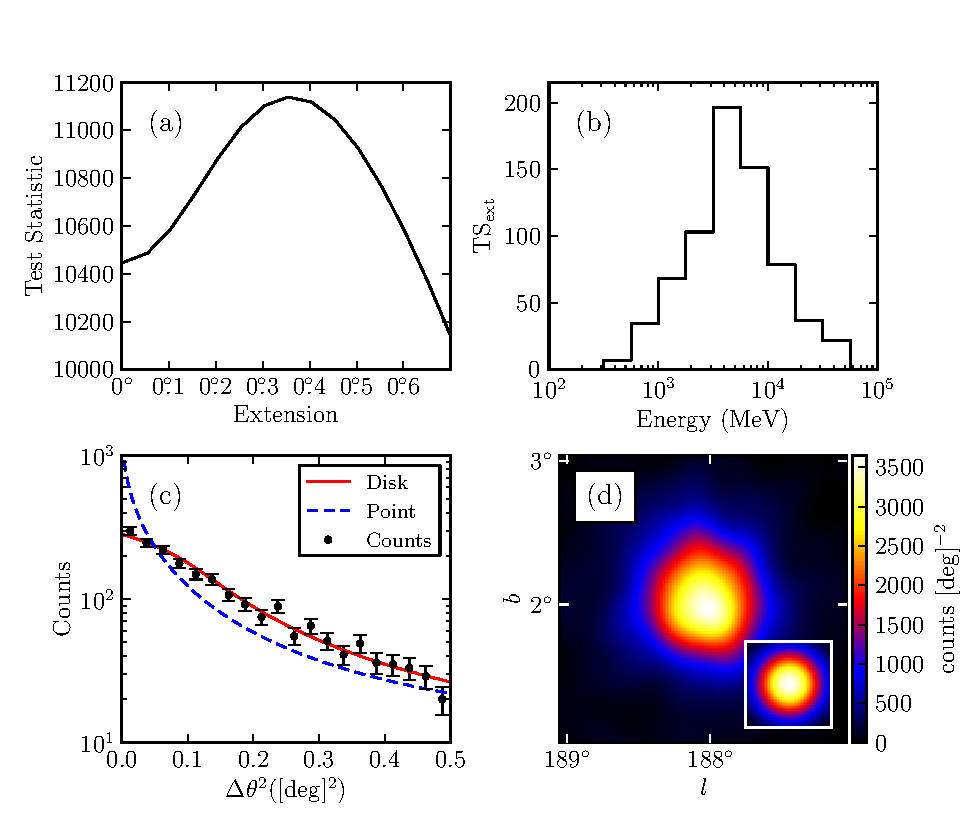
\includegraphics{ic443_plots/four_plots_ic443_color.pdf}
    \else
    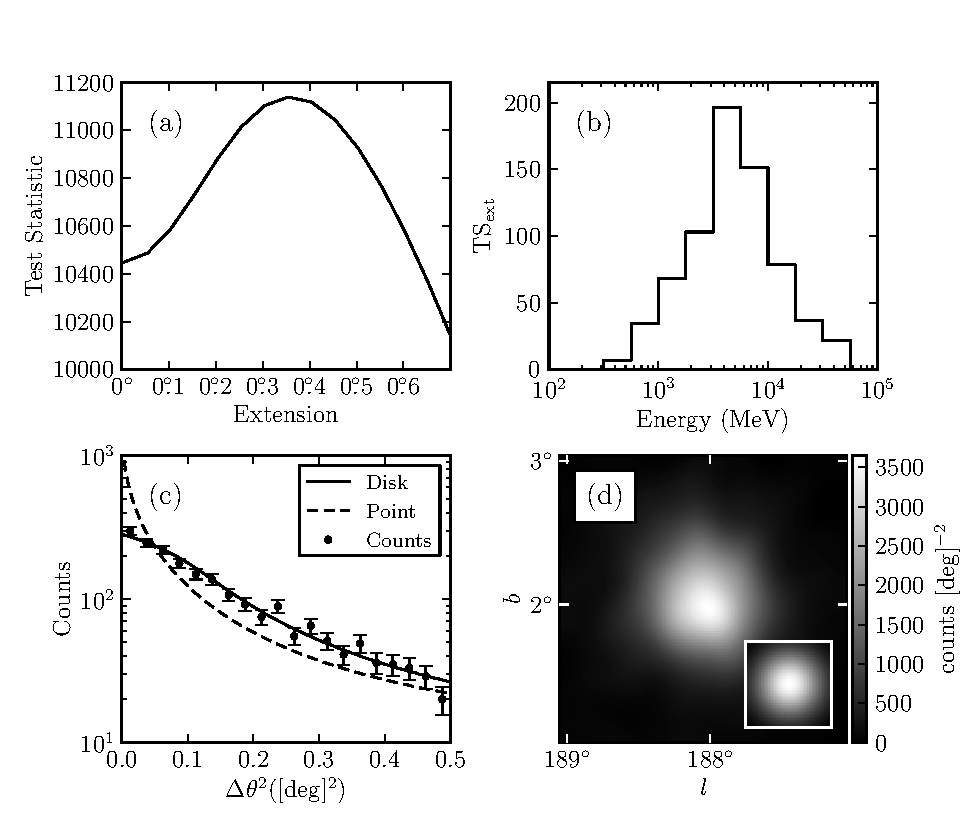
\includegraphics{ic443_plots/four_plots_ic443_bw.pdf}
    \fi
    % taken from /u/gl/lande/work/fermi/extended_catalog/2FGL/plots_for_paper/four_plots_ic443/v3/run.py
    \caption{
    Counts maps and TS profiles for the SNR IC~443. (a) \ts
    vs. extension of the source. (b) \tsext for individual energy
    bands. (c) observed radial profile of counts in comparison to the
    expected profiles for a spatially extended source (solid and colored
    red in the online version) and for a point-like source (dashed and colored
    blue in the online version).  (d) smoothed counts map after subtraction
    of the diffuse emission compared to the smoothed
    LAT PSF (inset). Both were smoothed by a 0\fdg1 2D Gaussian kernel.
    Plots (a),
    (c), and (d) use only 
    photons with energies between
    1 \gev and 100 \gev.  Plots (c) and (d) include
    only photons which converted in the front part of the tracker and
    have an improved angular resolution \citep{atwood_2009a_large-telescope}.
    }
    \figlabel{four_plots_ic443}
\end{figure}


We estimate the error on the extension of a source by fixing
the position of the source and varying the extension until the
log of the likelihood has decreased by 1/2, corresponding to a $1\sigma$ error
\citep{eadie_1971a_statistical-methods}.  \figref{four_plots_ic443}
demonstrates this method by showing the change in the log of the
likelihood when 
varying the modeled extension of the SNR IC~443.  The localization
error is calculated by fixing the extension and spectrum of the source
to their best fit values and then
fitting the log of the likelihood to
a 2D Gaussian as a function
of position. This localization error algorithm is further described in
\cite{nolan_2012_fermi-large}.

\subsection{\gtlike Analysis Validation}
\subseclabel{gtlike_crosscheck}

\pointlike is important for analyses of LAT data that require many iterations
such as source localization and extension fitting.  On the other hand,
because \gtlike makes fewer approximations in calculating the likelihood
we expect the spectral parameters found with \gtlike to be slightly more
accurate.  Furthermore, because \gtlike is the 
standard likelihood analysis package for LAT data, 
it has been more extensively validated for spectral analysis.
For those reasons, in the following analysis we used \pointlike to
determine the position and extension of a source and subsequently derived
the spectrum using \gtlike. Both \gtlike and \pointlike can be used to
estimate the statistical significance of the extension of a source and we
required that both methods agree for a source to be considered extended.
There was good agreement between the two methods.  Unless explicitly
mentioned, all \ts, \tsext, and spectral parameters were calculated using
\gtlike with the best-fit positions and extension found by \pointlike.


\subsection{Comparing Source Sizes}
\subseclabel{compare_source_size}


\clearpage
\begin{figure}
    \ifcolorfigure
      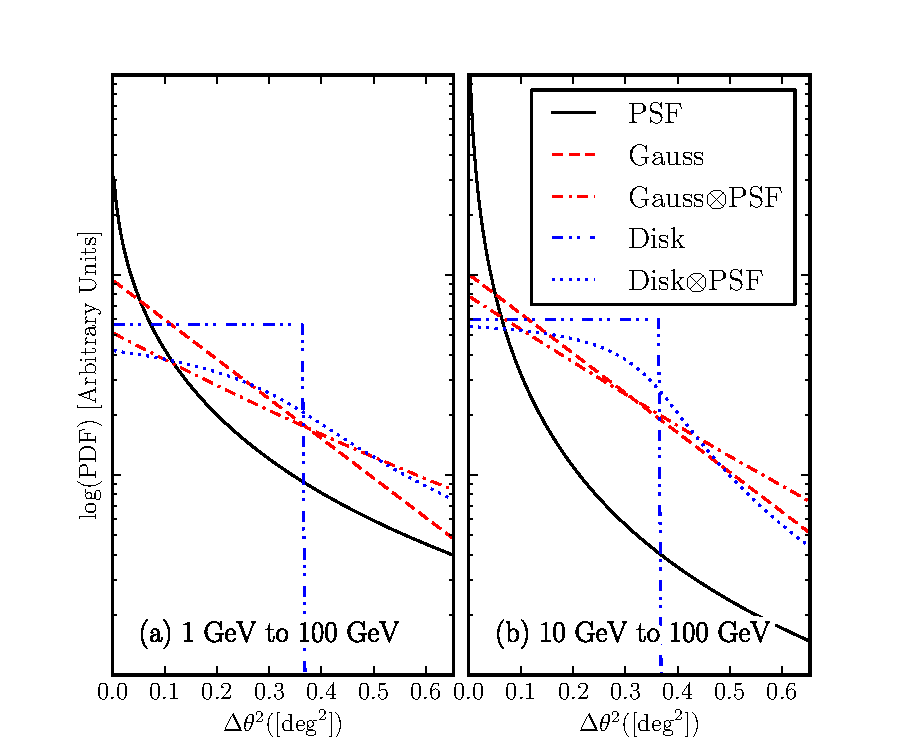
\includegraphics{mc_plots/compare_disk_gauss_color.pdf}
    \else
      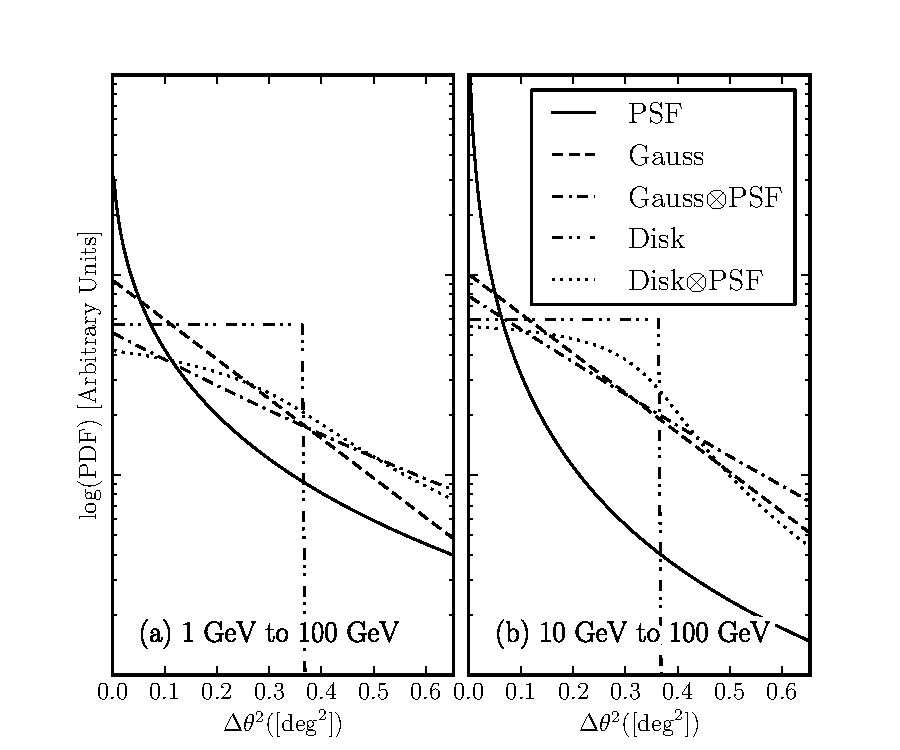
\includegraphics{mc_plots/compare_disk_gauss_bw.pdf}
    \fi
    \caption{
    A comparison of a 2D Gaussian and uniform disk spatial model
    of extended sources before and after convolving with the PSF for two
    energy ranges.  The solid black line is the PSF that would be observed
    for a power-law source of spectral index 2. The dashed line
    and the dash-dotted lines are 
    the brightness profile of a Gaussian with $\rsixeight=0\fdg5$
    and the convolution of this profile with the LAT PSF respectively
    (colored red in the online version).
    The dash-dot-dotted and the dot-dotted lines are the brightness profile
    of a uniform disk with $\rsixeight=0\fdg5$ and the convolution
    of this profile with the LAT PSF respectively (colored blue in the online version).
    }\figlabel{compare_disk_gauss}
  \end{figure}


We considered two models for the
surface brightness profile for extended sources: a 2D Gaussian model
\begin{equation}\eqnlabel{gauss_pdf}
  I_\text{Gaussian}(x,y)=\tfrac{1}{2\pi\sigma^2}\exp\left(-(x^2+y^2)/2\sigma^2\right)
\end{equation}
or a uniform disk model
\begin{equation}\eqnlabel{disk_pdf}
  I_\text{disk}(x,y)=
  \begin{cases}
    \frac{1}{\pi\sigma^2} & x^2+y^2\le\sigma^2 \\
    0                      & x^2+y^2>\sigma^2.
  \end{cases}
\end{equation}
Although these shapes are significantly different,
\figref{compare_disk_gauss} shows that, after convolution with the
LAT PSF, their PDFs are similar for a source that has a 0\fdg5 radius
typical of LAT-detected extended sources.  To allow a valid comparison
between the Gaussian and the uniform disk models,
we define the source size as the radius containing 68\% of the
intensity ($\rsixeight$). 
By direct integration, we find
\begin{align}
\rsixeight_\text{,Gaussian}=&1.51\sigma, \\
\rsixeight_\text{,disk}=&0.82\sigma, 
\end{align}
where $\sigma$ is defined
in \eqnref{gauss_pdf} and \eqnref{disk_pdf} respectively.
For the example above, $\rsixeight=0\fdg5$ so $\sigma_\text{disk}=0.61\degree$
and $\sigma_\text{Gaussian}=0.33\degree$.

For sources that are comparable in size to the PSF,
the differences in the PDF for
different spatial models are lost in the noise and the LAT is not sensitive
to the detailed spatial structure of these sources.  
In \subsecref{bias_wrong_spatial_model}, we perform a dedicated Monte Carlo simulation
that shows there is little bias due to incorrectly modeling the spatial structure
of an extended source.
Therefore, in our search for extended sources we use only a radially-symmetric uniform
disk spatial model. Unless otherwise noted,
we quote the radius to the edge ($\sigma$) as the size of the source.

\section{Validation of the TS Distribution}
\seclabel{validate_ts}

\subsection{Point-like Source Simulations Over a Uniform Background}
\subseclabel{monte_carlo_validation}

We tested the theoretical distribution for \tsext
to evaluate the false detection probability for measuring source extension.
To do so, we tested simulated point-like sources for extension. 
\cite{mattox_1996_likelihood-analysis}
discuss that the \ts distribution for a likelihood-ratio test
on the existence of a source at a given position is
\begin{equation}\eqnlabel{ts_ext_distribution}
  P(\ts)=\tfrac{1}{2}(\chi^2_1(\ts)+\delta(\ts)),
\end{equation}
where $P(\ts)$ is the probability density to get a particular value of TS,
$\chi^2_1$ is the chi-squared distribution with one degree of freedom, and
$\delta$ is the Dirac delta function.
The particular form of \eqnref{ts_ext_distribution} is due to the
null hypothesis (source flux $\Phi=0$) residing on the edge of parameter
space and the model hypothesis adding a single degree of freedom (the source flux).
It leads to the often quoted result $\sqrt{TS}=\sigma$, where 
$\sigma$ here refers to the significance of the detection. It is plausible
to expect a similar distribution for the TS in the test for
source extension since the same conditions apply (with the source flux
$\Phi$ replaced by the source radius $r$ and $r<0$ being unphysical).
To verify \eqnref{ts_ext_distribution}, we evaluated the
empirical distribution function of \tsext computed from simulated sources.

We simulated point-like sources with various spectral forms using
the LAT on-orbit simulation tool
\gtobssim\footnote{\gtobssim is distributed publicly by the FSSC.} and fit the sources
with \pointlike using both point-like
and extended source hypotheses.  These point-like sources were simulated with a power-law
spectral model with integrated fluxes above 100 \mev ranging from $3\times10^{-9}$ 
to $1\times10^{-5}$ \fluxunits and spectral
indices ranging from 1.5 to 3.  These values
were picked to represent typical parameters of LAT-detected
sources. The point-like sources were simulated on top of an isotropic
background with a power-law spectral model with
integrated flux above 100 \mev of $1.5\times10^{-5}$ \fluxunits sr$^{-1}$
and spectral index 2.1.
This was
taken to be the same as the isotropic spectrum measured by EGRET
\citep{sreekumar_1998a_egret-observations}.  This spectrum is comparable
to the high-latitude background intensity seen by the LAT.
The Monte Carlo simulation was performed
over a one-year observation period using a representative 
spacecraft orbit and livetime.
The reconstruction was performed
using the P7\_V6 Source class event selection and IRFs \citep{ackermann_2012a_fermi-large}. For each 
significantly detected point-like source ($\ts\ge25$), we used \pointlike
to fit the source as an extended source and calculate \tsext.
This entire procedure was performed twice, once fitting in the 1 \gev
to 100 \gev energy range and once fitting in the 10 \gev to 100 \gev
energy range.


\clearpage
\begin{figure}
    \ifcolorfigure
    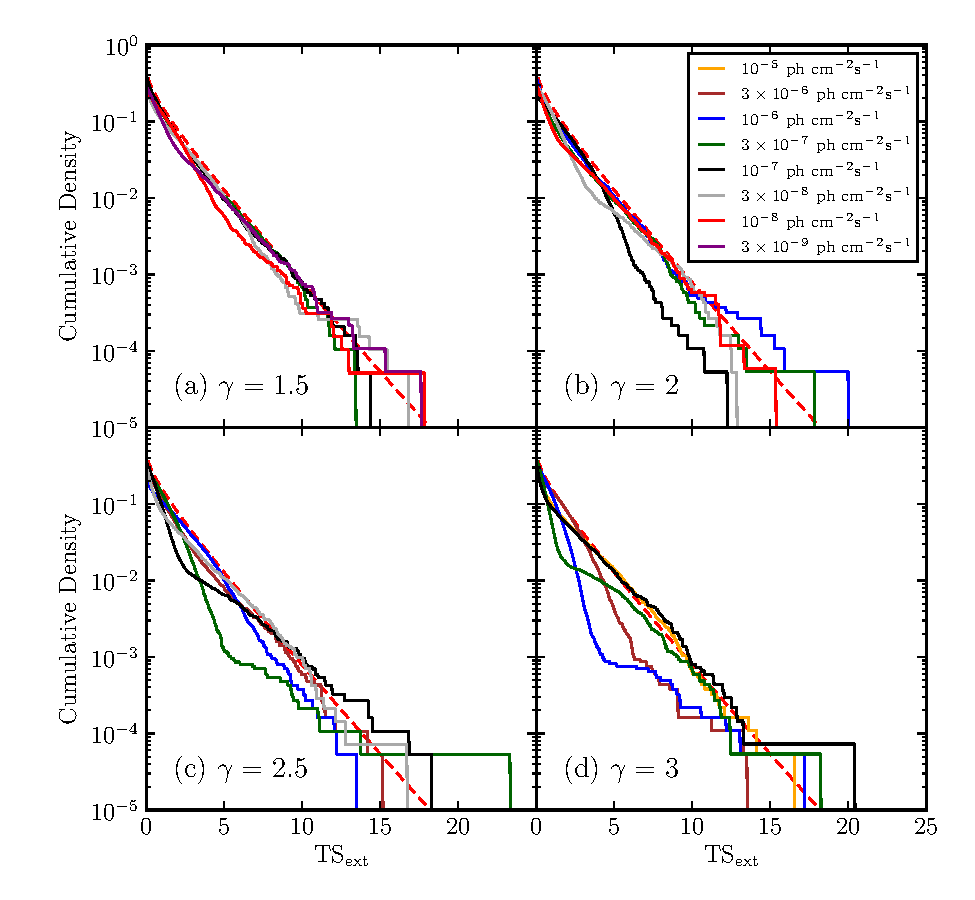
\includegraphics{mc_plots/ts_ext_emin_1000_color.pdf}
    \else
    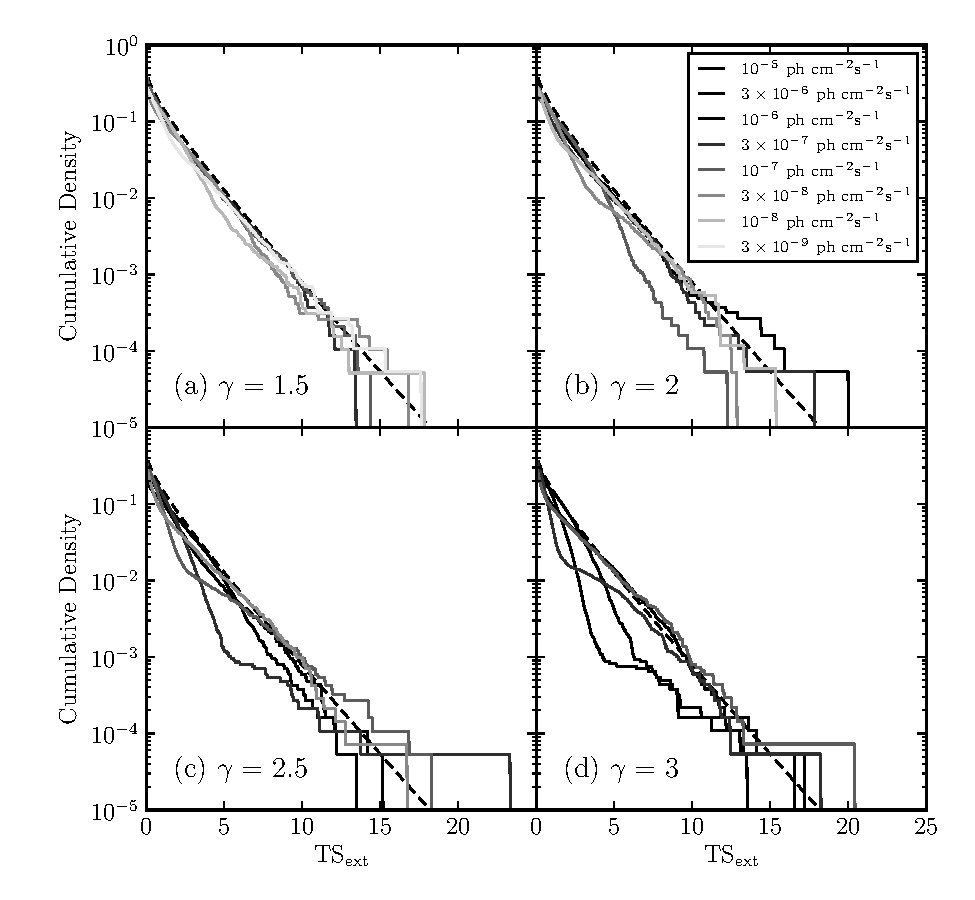
\includegraphics{mc_plots/ts_ext_emin_1000_bw.pdf}
    \fi
    \caption{
    Cumulative distribution of the TS for the extension test when fitting
    simulated point-like sources in the 1 GeV to 100 GeV energy range.
    The four plots
    represent simulated sources of different spectral indices and
    the different lines (colored in the online version) 
    represent point-like sources with different 100 \mev
    to 100 \gev integral fluxes.  The dashed line (colored red)
    is the cumulative
    density function of \eqnref{ts_ext_distribution}.
    }\figlabel{ts_ext_mc_1000}
  \end{figure}


\clearpage
\begin{figure}
    \ifcolorfigure
    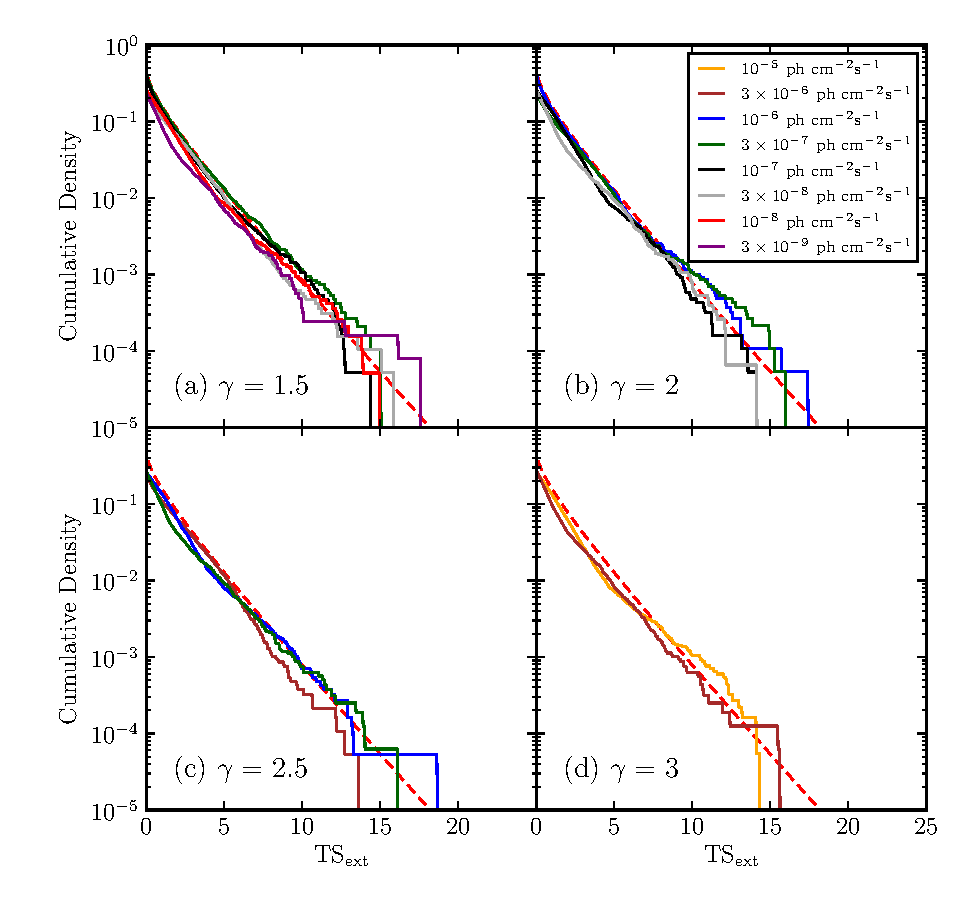
\includegraphics{mc_plots/ts_ext_emin_10000_color.pdf}
    \else
    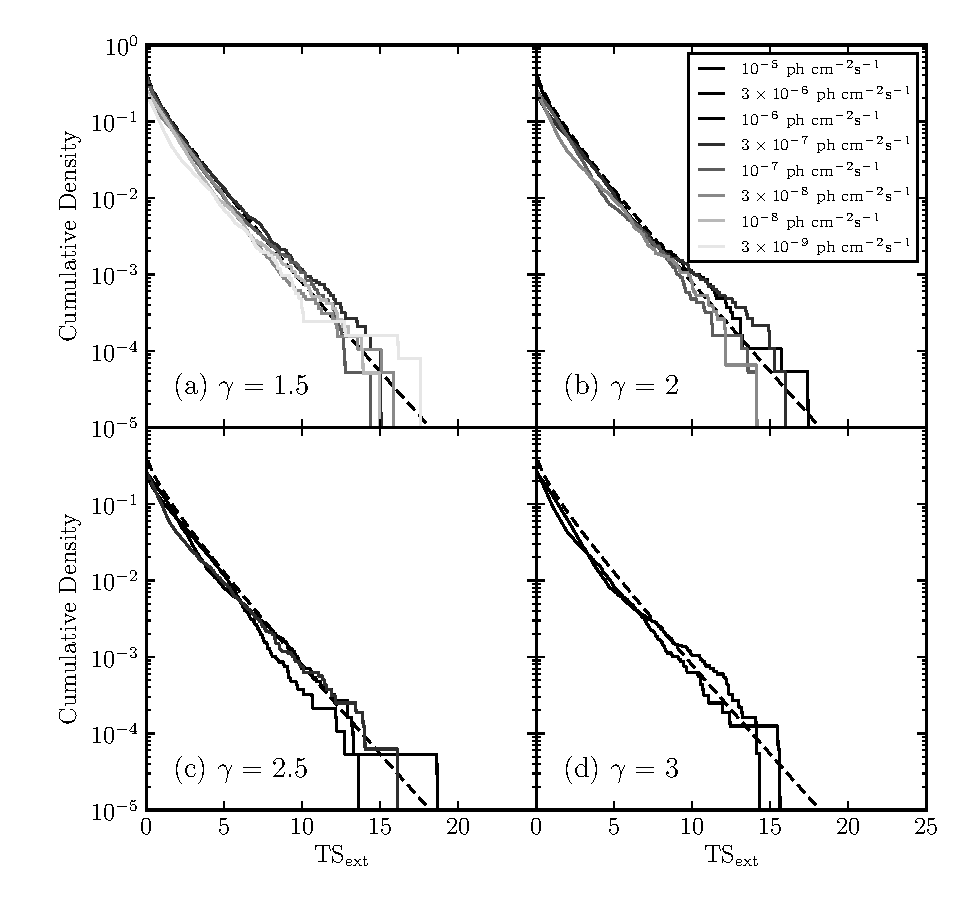
\includegraphics{mc_plots/ts_ext_emin_10000_bw.pdf}
    \fi
    \caption{
    The same plot as \figref{ts_ext_mc_1000} but fitting in the 10 \gev to 100 \gev energy 
    range.
    }\figlabel{ts_ext_mc_10000}
  \end{figure}



\clearpage
\begin{deluxetable}{rrrrrr}
\tabletypesize{\scriptsize}
\tablecaption{Monte Carlo Spectral Parameters
\tablabel{ts_ext_num_sims}
}
\tablecolumns{6}
\tablewidth{0pt}
\tablehead{
\colhead{Spectral Index}&
\colhead{Flux\tablenotemark{(a)}}&
\colhead{$N_{1-100\gev}$}&
\colhead{$\langle\ts\rangle_{1-100\gev}$}&
\colhead{$N_{10-100\gev}$}&
\colhead{$\langle\ts\rangle_{10-100\gev}$}\\
\colhead{}&
\colhead{(\fluxunits)}&
\colhead{}&
\colhead{}&
\colhead{}&
\colhead{}
}

\startdata
\multicolumn{6}{c}{Isotropic Background} \\
\hline
      1.5 &  $3\times 10^{-7}$ &           18938 &  22233    &     18938   &    8084     \\
          &          $10^{-7}$ &           19079 &   5827    &     19079   &    2258     \\
          &  $3\times 10^{-8}$ &           19303 &   1276    &     19303   &     541     \\
          &          $10^{-8}$ &           19385 &    303    &     19381   &     142     \\
          &  $3\times 10^{-9}$ &           18694 &     62    &     12442   &      43     \\
      \hline
        2 &          $10^{-6}$ &           18760 &  22101    &     18760   &    3033     \\
          &  $3\times 10^{-7}$ &           18775 &   4913    &     18775   &     730     \\
          &          $10^{-7}$ &           18804 &   1170    &     18803   &     192     \\
          &  $3\times 10^{-8}$ &           18836 &    224    &     15256   &      50     \\
          &          $10^{-8}$ &           17060 &     50    &   \nodata   & \nodata     \\
      \hline
      2.5 &  $3\times 10^{-6}$ &           18597 &  19036    &     18597   &     786    \\
          &          $10^{-6}$ &           18609 &   4738    &     18608   &     208    \\
          &  $3\times 10^{-7}$ &           18613 &    954    &     15958   &      53    \\
          &          $10^{-7}$ &           18658 &    203    &   \nodata   & \nodata    \\
          &  $3\times 10^{-8}$ &           14072 &     41    &   \nodata   & \nodata    \\
      \hline                                                
        3 &          $10^{-5}$ &           18354 &  19466    &     18354   &     215    \\
          &  $3\times 10^{-6}$ &           18381 &   4205    &     15973   &      54    \\
          &          $10^{-6}$ &           18449 &    966    &   \nodata   & \nodata    \\
          &  $3\times 10^{-7}$ &           18517 &    174    &   \nodata   & \nodata    \\
          &          $10^{-7}$ &           13714 &     41    &   \nodata   & \nodata    \\
\cutinhead{Galactic Diffuse and Isotropic Background\tablenotemark{(b)}}
      1.5 &  $2.3\times 10^{-8}$ &           90741 &     63    &   \nodata   & \nodata     \\
        2 &  $1.2\times 10^{-7}$ &           92161 &     60    &   \nodata   & \nodata     \\
      2.5 &  $4.5\times 10^{-7}$ &           86226 &     47    &   \nodata   & \nodata    \\
        3 &  $2.0\times 10^{-6}$ &           94412 &     61    &   \nodata   & \nodata    \\
\enddata

\tablenotetext{(a)}{Integral 100 \mev to 100 \gev flux.}
\tablenotetext{(b)}{
For the Galactic simulations, the quoted fluxes are
the fluxes for sources placed 
in the Galactic center. The actual fluxes are scaled by \eqnref{scale_flux_by_background}.
}

\tablecomments{
    A list of the spectral models of the simulated point-like sources
    which were tested for extension.  For each model, the number of
    statistically independent simulations and the average value of \ts is
    also tabulated.  
    The top rows are the simulations on top of an isotropic background and
    the bottom rows are the simulations on top of the Galactic diffuse and isotropic
    background.
}
\end{deluxetable}


For each set of spectral parameters, $\sim20,000$ statistically independent
simulations were performed. For lower-flux spectral models, many of the
simulations left the source insignificant ($\ts<25$)
and were discarded.  \tabref{ts_ext_num_sims}
shows the different spectral models used in our study as well as the
number of simulations and the average point-like source
significance.  The cumulative density of \tsext is plotted in
\figref{ts_ext_mc_1000} and \figref{ts_ext_mc_10000} 
and compared to the $\chi^2_1/2$ distribution of
\eqnref{ts_ext_distribution}.

Our study shows broad agreement between simulations and
\eqnref{ts_ext_distribution}. To the extent that there is
a discrepancy, the simulations tended to produce smaller than expected
values of \tsext which would make the formal significance conservative.
Considering the distribution in \figref{ts_ext_mc_1000} and
\figref{ts_ext_mc_10000}, the choice of a threshold \tsext set to 16
(corresponding to a formal $4\sigma$ significance) is reasonable.


\subsection{Point-like Source Simulations Over a Structured Background}
\subseclabel{validation_over_plane}

We performed a second set of simulations to show that the theoretical distribution
for \tsext is still preserved when the point-like sources are present over
a highly-structured diffuse background.
Our simulation setup was the same as above except that the sources were
simulated on top of and analyzed assuming the presence of the standard
Galactic diffuse and isotropic background models used in 2FGL.  In our
simulations, we selected our sources to have random positions on the sky
such that they were within 5\degree of the Galactic plane. This probes the 
brightest and most strongly contrasting areas of the Galactic background.

To limit the number of tests, we selected only one flux
level for each of the four spectral indices and we performed
this test only in the 1 \gev to 100 \gev energy range. 
As described below, the fluxes were selected so that $\ts\sim50$. We do not
expect to be able to spatially resolve sources 
at lower fluxes than these, and the results for much brighter sources
are less likely to be affected by the 
structured background.

Because the Galactic diffuse emission is highly structured with
strong gradients, the point-source
sensitivity can vary significantly across the Galactic plane.
To account for this, we scaled the flux (for a given spectral index)
so that the source always has approximately the same signal-to-noise ratio:
\begin{equation}
  \eqnlabel{scale_flux_by_background}
  F(\vec{x}) = F(\text{GC}) \times \left(
  \frac{B(\vec{x})}{B(\text{GC})}\right)^{1/2}.
\end{equation}
Here, $\vec{x}$ is the position of the simulated source, $F$ is the integral
flux of the source from 100 \mev to 100 \gev, $F(\text{GC})$
is the same quantity if the source was at the Galactic center, $B$
is the integral of the Galactic diffuse and isotropic emission
from 1 \gev to 100 \gev at the position of the source, and $B(\text{GC})$ is the same quantity
if the source was at the Galactic center.  For the four spectral models,
\tabref{ts_ext_num_sims} lists $F(\text{GC})$ and the average value of \ts.

\clearpage
\begin{figure}
    \ifcolorfigure
    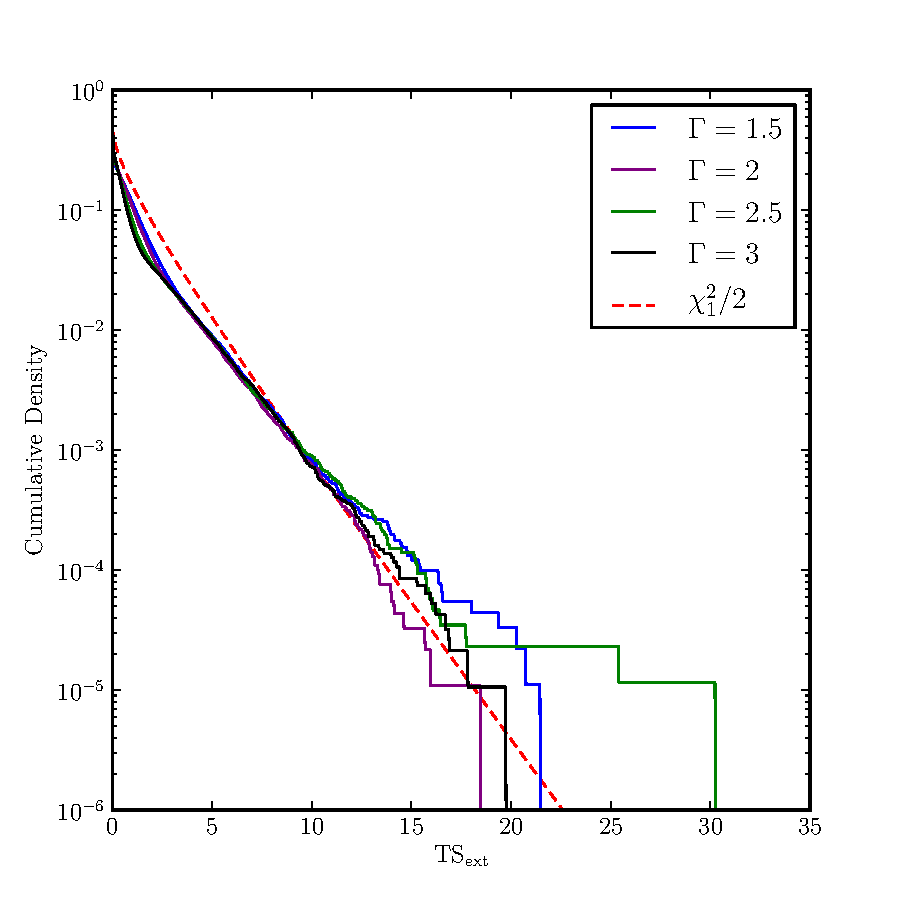
\includegraphics{mc_plots/plot_tsext_plane_color.pdf}
    \else
    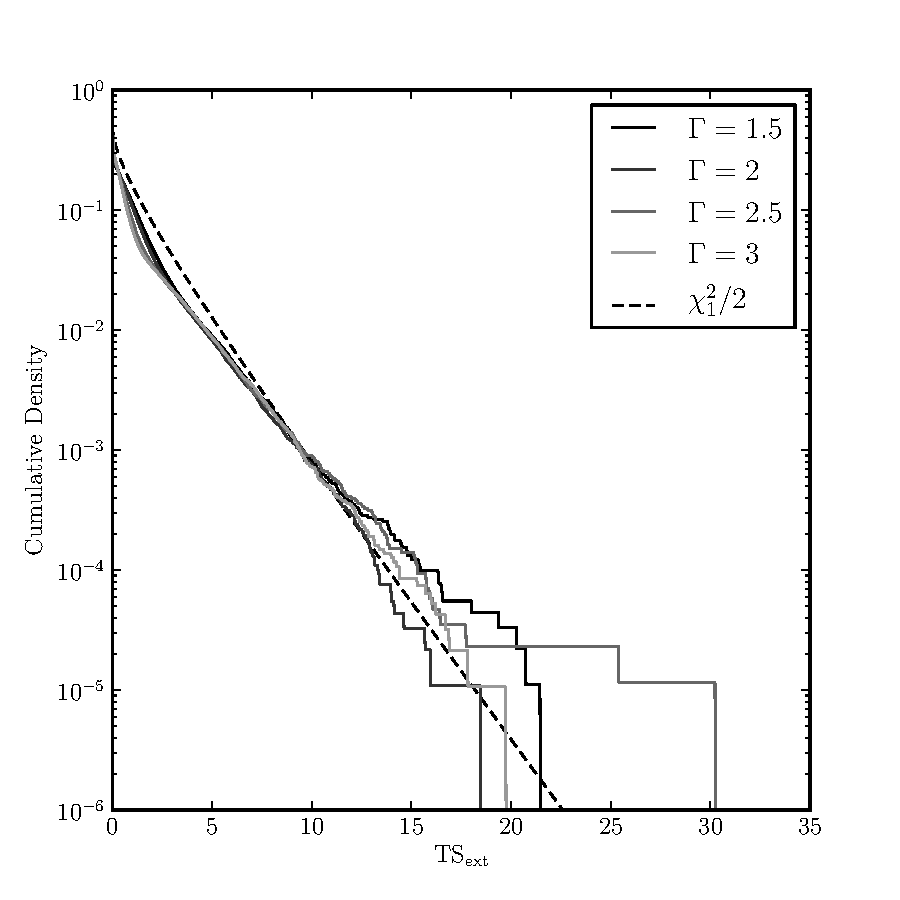
\includegraphics{mc_plots/plot_tsext_plane_bw.pdf}
    \fi
    \caption{
    Cumulative distribution of \tsext
    for sources simulated on top of the Galactic diffuse and isotropic background.
    }\figlabel{tsext_plane_plot}
  \end{figure}



For each spectrum, we performed $\sim90,000$ simulations.
\figref{tsext_plane_plot} shows the cumulative density
of \tsext for each spectrum. For small values of \tsext,
there is good agreement between the simulations and
theory.  For the highest values of \tsext, there is possibly
a small discrepancy, but the discrepancy is not statistically significant.
Therefore, we are confident we can use \tsext as a robust measure of
statistical significance when testing LAT-detected sources for extension.

\subsection{Extended Source Simulations Over a Structured Background}
\subseclabel{bias_wrong_spatial_model}

We also performed a Monte Carlo study to show that incorrectly modeling the
spatial extension of an extended source does not substantially bias
the spectral fit of the source, although it does alter the value of the \ts.
To assess this, we simulated the spatially extended ring-type SNR W44.
We selected W44 because it is the most significant extended source detected by the LAT 
that has a non-radially symmetric photon distribution \citep{abdo_2010a_gamma-ray-emission}. 

W44 was simulated with a power-law spectral model with an integral flux
of $7.12\times10^{-8}$ \fluxunits in the energy range from 1 \gev to 100
\gev and a spectral index of 2.66 (see \secref{validate_known}).

W44 was simulated with the elliptical ring spatial model described in
\cite{abdo_2010a_gamma-ray-emission}. For reference, the ellipse has a semi-major axis of 0\fdg3,
a semi-minor axis of 0\fdg19, a position angle of $147\degree$
measured East of celestial North, and the ring's inner radius is 75\% of
the outer radius.

We used a simulation setup similar to that described in
\subsecref{validation_over_plane}, but the simulations
were over the 2-year interval of the 2FGL catalog.
In the simulations, 
we did not include the finite energy resolution of the LAT
to isolate any effects due to changing the assumed spatial model. 
The fitting code we use also ignores this energy dispersion and the
potential bias introduced by this will be discussed in an upcoming paper
by the LAT collaboration \citep{ackermann_2012a_fermi-large}.
In total, we performed 985 independent simulations.

The simulated sources were fit using a point-like spatial model,
a radially-symmetric Gaussian spatial model, a uniform disk spatial model, 
an elliptical disk spatial model, and finally with an elliptical
ring spatial model.
We obtained the best fit spatial parameters using \pointlike and, 
with these parameters, obtained the best fit spectral parameters 
using \gtlike. 

\clearpage
\begin{figure}
    \ifcolorfigure
    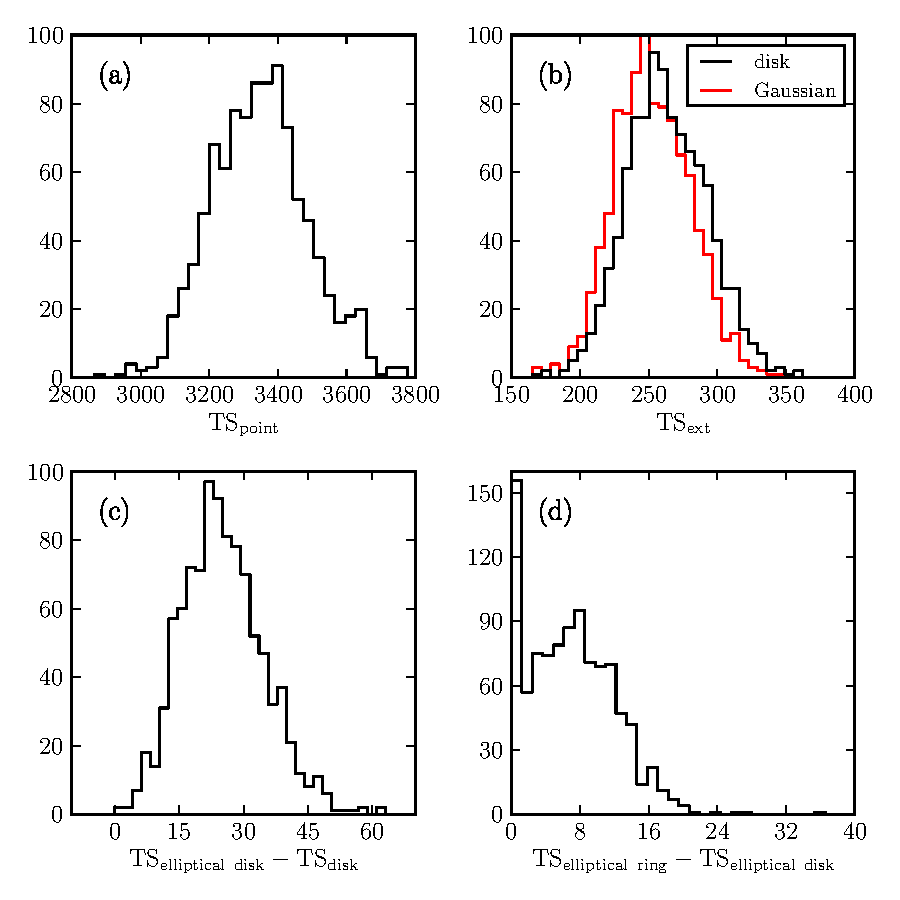
\includegraphics{mc_plots/ts_comparison_w44sim_color.pdf}
    \else
    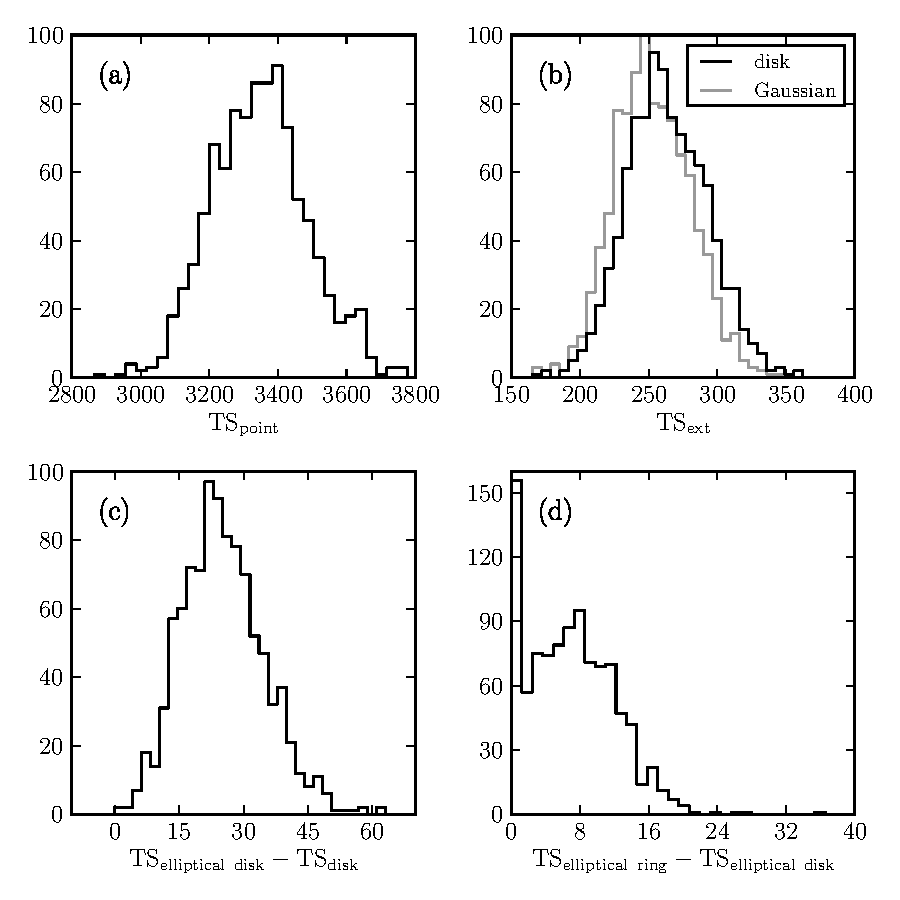
\includegraphics{mc_plots/ts_comparison_w44sim_bw.pdf}
    \fi
    \caption{
    The distribution of \ts values when fitting 985 statistically
    independent simulations of W44. (a) is the distribution of \ts values
    when fitting W44 as a point-like source and (b) is the
    distribution of \tsext when fitting the source with a uniform disk or a 
    radially-symmetric Gaussian
    spatial model. (c) is the distribution of the change in TS when
    fitting the source with an elliptical disk spatial model compared to
    fitting it with a radially-symmetric disk spatial model and (d) 
    when fitting the source with an elliptical ring spatial model compared
    to an elliptical disk spatial model.
    }\figlabel{ts_comparison_w44sim}
\end{figure}


\figref{ts_comparison_w44sim}a 
shows that
the significance of W44 in the simulations is very large ($\ts\sim3500$) 
for a model with a point-like source hypothesis.
\figref{ts_comparison_w44sim}b shows that 
the significance of the spatial extension is also large
($\tsext\sim250$).  
On average \tsext is somewhat larger when fitting
the sources with more accurate spatial models.  This shows that
assuming an incorrect spatial model will cause the source's
significance to be underestimated.  \figref{ts_comparison_w44sim}c
shows that the sources were fit better when assuming an elliptical
disk spatial model compared to a uniform disk spatial model
($\ts_\text{elliptical\ disk}-\ts_\text{disk}\sim30$).  Finally,
\figref{ts_comparison_w44sim}d shows that the sources were
fit somewhat better assuming an elliptical ring spatial model
compared to an elliptical disk spatial model ($\ts_\text{elliptical\
ring}-\ts_\text{elliptical\ disk}\sim9$). This shows that the LAT has
some additional power to resolve substructure in bright extended sources.

\clearpage
\begin{figure}
    \ifcolorfigure
    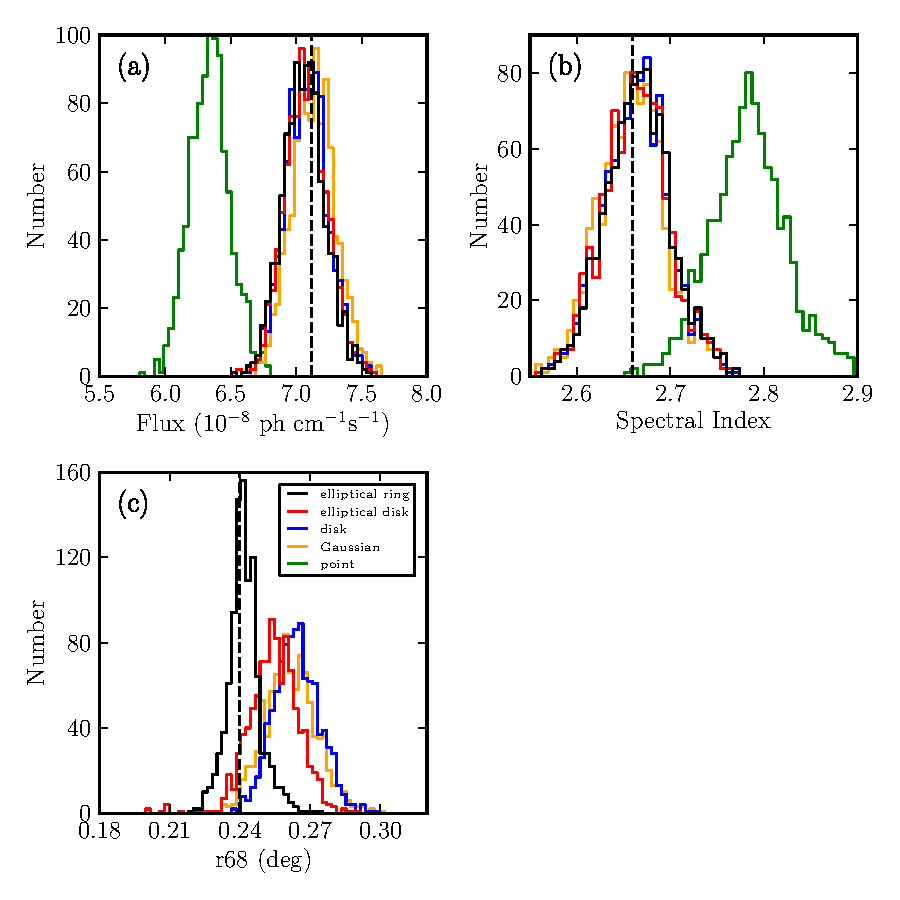
\includegraphics{mc_plots/bias_w44sim_color.pdf}
    \else
    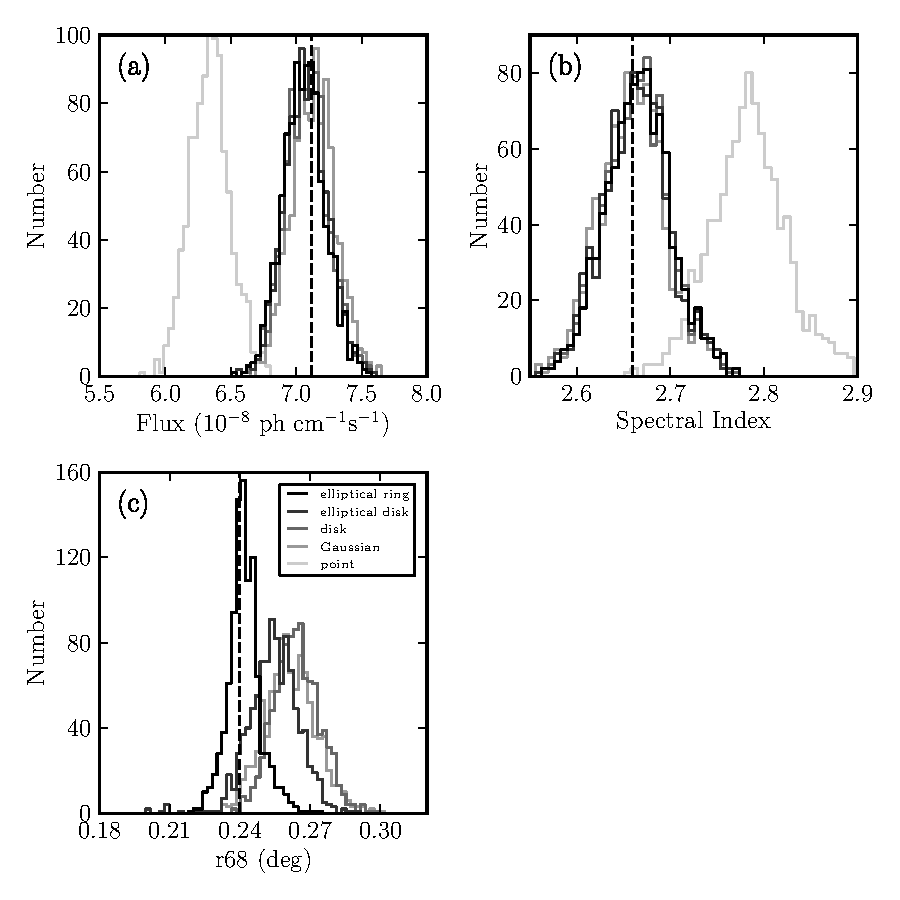
\includegraphics{mc_plots/bias_w44sim_bw.pdf}
    \fi
    \caption{
    The distribution of fit parameters
    for the Monte Carlo simulations of W44.
    The plots show the distribution of 
    best fit (a) flux (b) spectral index and (c) 68\% containment
    radius. The dashed vertical lines represent
    the simulated values of the parameters.
    }\figlabel{bias_w44sim}
\end{figure}



\figref{bias_w44sim}a and \figref{bias_w44sim}b clearly show that
no significant bias is introduced by modeling the source as extended
but with an inaccurate spatial model, while a point-like source modeling
results in a $\sim10\%$ and $\sim0.125$ bias in the fit flux and index,
respectively.  
Furthermore, \figref{bias_w44sim}c shows that the \rsixeight estimate of
the extension size is very mildly biased ($\sim10\%$) toward higher values
when inaccurate spatial models are used, and thus represents a reasonable
measurement of the true 68\% containment radius for the source.
For the elliptical spatial models, \rsixeight is computed by numeric integration.


\section{Extended Source Detection Threshold}
\subseclabel{extension_sensitivity}

We calculated the LAT flux 
threshold to detect spatial extent. We define the detection threshold as the flux at
which the value of $\tsext$ averaged over many statistical realizations is
$\langle\tsext\rangle=16$ 
(corresponding to a formal $4\sigma$ significance)
for a source of a given extension.

We used a simulation setup similar to that described in
\subsecref{monte_carlo_validation}, but instead of point-like sources
we simulated extended sources with radially-symmetric uniform disk spatial 
models. Additionally, we simulated our sources over the two-year
time range included in the 2FGL catalog.  For each extension and spectral index,
we selected a flux range which bracketed $\tsext=16$ and performed an
extension test for $>100$ independent realizations of ten fluxes in
the range.  We calculated $\langle\tsext\rangle=16$ by fitting a line
to the flux and $\tsext$ values in the narrow range.

\clearpage
\begin{figure}
    \ifcolorfigure
    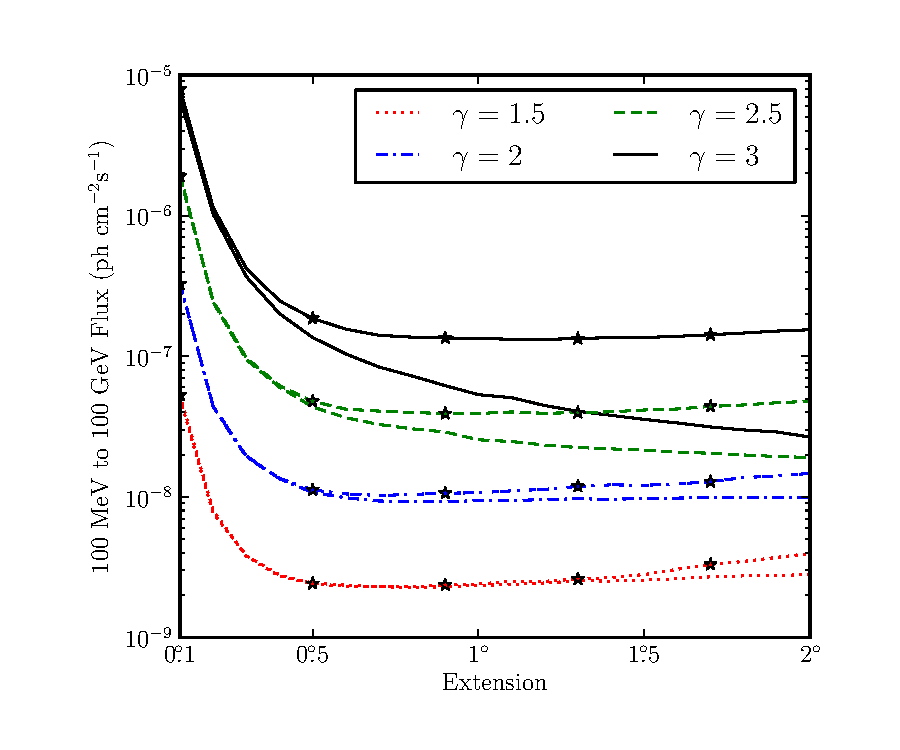
\includegraphics{mc_plots/index_sensitivity_color.pdf}
    \else
    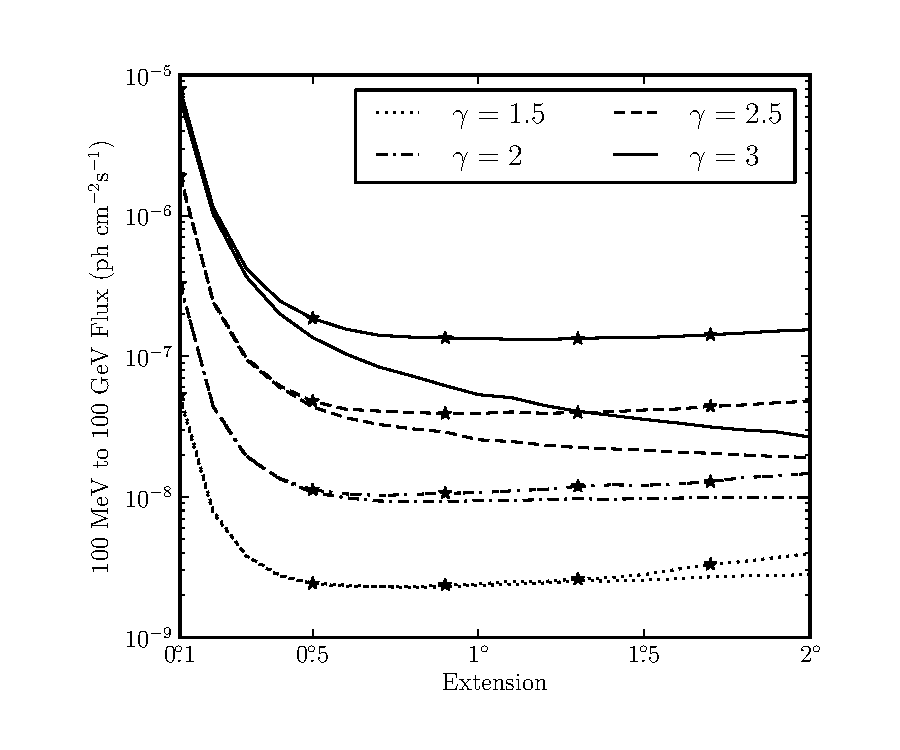
\includegraphics{mc_plots/index_sensitivity_bw.pdf}
    \fi
    \caption{
    The detection threshold to resolve an
    extended source with a uniform disk model for a two-year exposure.  All sources have an
    assumed power-law spectrum and the different line styles (colors in
    the electronic version) correspond to different simulated spectral
    indices.  The lines with no markers correspond to the detection
    threshold using photons with energies between 100 \mev and 100 \gev,
    while the lines with star-shaped markers correspond to the threshold
    using photons with energies between 1 \gev and 100 \gev.
    }\figlabel{index_sensitivity}
  \end{figure}


\figref{index_sensitivity} shows the threshold for sources of four
spectral indices from 1.5 to 3 and extensions varying from $\sigma=0\fdg1$
to $2\fdg0$.  
The threshold is high for small extensions when the
source is 
small compared to the size of the PSF. 
It drops quickly with increasing source size and reaches
a minimum around 0\fdg5. 
The threshold increases
for large extended sources because the source becomes
increasingly diluted by the background.
\figref{index_sensitivity} shows
the threshold using photons with energies between 100 \mev and 100 \gev
and also using only photons with energies between 1 \gev and 100 \gev.
Except for very large or very soft
sources, the threshold is
not substantially improved by including photons with energies between 100 \mev and
1 \gev.  This is also demonstrated in \figref{four_plots_ic443}
which shows \tsext for the SNR IC~443 computed independently in twelve
energy bins between 100 \mev and 100 \gev. For IC~443, which has a
spectral index $\sim2.4$ and an extension $\sim0\fdg35$, 
almost the entire 
increase in likelihood from optimizing the source extent in the model
comes
from energies above 1 \gev.  Furthermore, other systematic errors
become increasingly large at low energy. For our extension search
(\secref{extended_source_search_method}),
we therefore used only photons with energies above 1 \gev.


  \thispagestyle{empty}
\begin{deluxetable}{rr|rrrrrrrrrrrrrrrrrrrrr}
\tablecolumns{22}
\tabletypesize{\scriptsize}
\rotate
\tablewidth{0pt}
\tablecaption{Extension Detection Threshold
\tablabel{all_sensitivity_table}
}
\tablehead{
\colhead{$\gamma$}&       
\colhead{BG}&
\colhead{$0.1$}&
\colhead{$0.2$}&
\colhead{$0.3$}&
\colhead{$0.4$}&
\colhead{$0.5$}&
\colhead{$0.6$}&
\colhead{$0.7$}&
\colhead{$0.8$}&
\colhead{$0.9$}&
\colhead{$1.0$}&
\colhead{$1.1$}&
\colhead{$1.2$}&
\colhead{$1.3$}&
\colhead{$1.4$}&
\colhead{$1.5$}&
\colhead{$1.6$}&
\colhead{$1.7$}&
\colhead{$1.8$}&
\colhead{$1.9$}&
\colhead{$2.0$}
}
\startdata
\multicolumn{22}{c}{E$>$1 \gev} \\
\hline
     1.5 &      $1\times$ &      148.1 &       23.3 &       11.3 &        8.0 &        7.2 &        6.9 &        6.7 &        6.8 &        7.1 &        7.4 &        7.6 &        7.9 &        8.1 &        8.5 &        9.2 &        9.9 &        9.1 &        9.2 &        9.0 &       10.3 \\
         &     $10\times$ &      148.4 &       29.0 &       18.7 &       15.2 &       15.4 &       15.0 &       16.1 &       16.0 &       16.8 &       17.7 &       18.2 &       19.3 &       20.9 &       22.5 &       23.8 &       24.8 &       21.3 &       22.8 &       23.4 &       23.7 \\
         &    $100\times$ &      186.8 &       55.0 &       43.4 &       40.7 &       41.0 &       41.8 &       40.9 &       40.9 &       42.7 &       43.6 &       38.4 &       39.9 &       40.6 &       38.4 &       36.9 &       36.3 &       37.1 &       38.8 &       37.2 &       37.6 \\
       2 &      $1\times$ &      328.4 &       43.4 &       18.9 &       13.4 &       11.2 &       10.4 &       10.2 &       10.2 &       10.2 &       10.4 &       10.7 &       10.9 &       11.2 &       11.5 &       12.4 &       12.6 &       13.0 &       13.4 &       14.0 &       14.4 \\
         &     $10\times$ &      341.0 &       55.9 &       32.3 &       27.6 &       26.5 &       25.4 &       25.6 &       25.9 &       27.4 &       26.8 &       27.8 &       28.7 &       29.8 &       30.1 &       31.0 &       31.5 &       31.7 &       34.0 &       34.3 &       35.9 \\
         &    $100\times$ &      420.5 &      128.3 &       90.2 &       77.3 &       73.3 &       70.8 &       67.5 &       64.3 &       64.2 &       64.1 &       62.8 &       63.6 &       61.7 &       61.9 &       58.4 &       59.0 &       61.4 &       63.3 &       60.1 &       58.1 \\
     2.5 &      $1\times$ &      627.1 &       75.6 &       29.8 &       19.3 &       15.5 &       13.5 &       12.8 &       12.6 &       12.5 &       12.5 &       12.6 &       12.9 &       12.9 &       13.1 &       13.5 &       13.7 &       14.3 &       14.8 &       15.2 &       15.8 \\
         &     $10\times$ &      638.9 &       99.1 &       52.1 &       39.1 &       34.6 &       33.0 &       32.5 &       32.5 &       32.8 &       33.2 &       34.1 &       34.3 &       34.5 &       35.1 &       36.6 &       36.9 &       35.5 &       36.0 &       36.5 &       37.3 \\
         &    $100\times$ &      795.0 &      262.1 &      140.9 &      104.3 &       90.4 &       81.2 &       77.2 &       75.1 &       69.7 &       70.9 &       66.5 &       65.6 &       64.9 &       64.0 &       58.9 &       58.1 &       60.2 &       58.4 &       57.5 &       55.8 \\
       3 &      $1\times$ &      841.5 &      110.6 &       43.2 &       25.5 &       18.7 &       16.1 &       14.4 &       13.6 &       13.3 &       13.2 &       13.1 &       13.1 &       13.4 &       13.6 &       13.5 &       13.8 &       14.2 &       14.4 &       14.8 &       15.4 \\
         &     $10\times$ &      921.6 &      151.3 &       69.1 &       47.8 &       40.7 &       37.1 &       35.5 &       34.5 &       35.1 &       35.5 &       35.3 &       35.3 &       35.4 &       35.5 &       36.8 &       37.6 &       35.3 &       35.4 &       36.3 &       36.6 \\
         &    $100\times$ &     1124.1 &      282.9 &      181.1 &      119.8 &      100.7 &       91.1 &       84.3 &       77.9 &       73.3 &       71.8 &       67.6 &       66.4 &       65.5 &       63.9 &       59.0 &       58.6 &       58.8 &       57.5 &       55.4 &       54.4 \\
\cutinhead{E$>$10 \gev}
     1.5 &      $1\times$ &       44.6 &        8.0 &        4.3 &        3.2 &        2.7 &        2.6 &        2.5 &        2.5 &        2.4 &        2.5 &        2.5 &        2.6 &        2.7 &        2.8 &        2.9 &        2.9 &        3.1 &        3.2 &        3.3 &        3.4 \\
         &     $10\times$ &       45.2 &        9.2 &        5.8 &        5.0 &        4.9 &        4.9 &        5.0 &        5.2 &        5.3 &        5.7 &        5.9 &        6.3 &        6.6 &        6.5 &        6.8 &        7.6 &        7.8 &        8.2 &        8.5 &        8.7 \\
         &    $100\times$ &       47.3 &       13.4 &       11.6 &       10.6 &       10.8 &       10.8 &       12.0 &       12.7 &       13.2 &       13.7 &       15.3 &       16.1 &       17.2 &       18.2 &       18.9 &       19.5 &       20.4 &       21.0 &       21.7 &       22.9 \\
       2 &      $1\times$ &       49.7 &        8.4 &        4.4 &        3.3 &        2.8 &        2.6 &        2.6 &        2.6 &        2.6 &        2.6 &        2.7 &        2.7 &        2.8 &        2.9 &        3.0 &        3.2 &        3.2 &        3.4 &        3.5 &        3.5 \\
         &     $10\times$ &       48.6 &        9.5 &        6.0 &        5.2 &        5.0 &        5.2 &        5.2 &        5.3 &        5.4 &        5.8 &        6.4 &        6.6 &        7.0 &        7.1 &        7.5 &        8.0 &        8.3 &        8.6 &        9.0 &        9.2 \\
         &    $100\times$ &       51.8 &       14.7 &       11.8 &       11.5 &       11.5 &       11.9 &       13.2 &       14.0 &       14.3 &       15.3 &       16.2 &       16.9 &       18.4 &       19.2 &       19.8 &       21.0 &       22.0 &       22.8 &       23.2 &       24.3 \\
     2.5 &      $1\times$ &       53.1 &        9.1 &        4.5 &        3.3 &        2.8 &        2.7 &        2.6 &        2.5 &        2.5 &        2.6 &        2.7 &        2.7 &        2.8 &        2.8 &        2.9 &        3.1 &        3.2 &        3.3 &        3.5 &        3.6 \\
         &     $10\times$ &       53.7 &       10.5 &        6.3 &        5.4 &        5.1 &        5.1 &        5.3 &        5.4 &        5.7 &        6.0 &        6.3 &        6.6 &        6.8 &        6.9 &        7.5 &        8.1 &        8.3 &        8.6 &        8.9 &        9.2 \\
         &    $100\times$ &       57.0 &       15.6 &       12.7 &       11.9 &       11.8 &       12.2 &       13.1 &       14.3 &       14.6 &       15.2 &       16.3 &       17.0 &       18.8 &       19.2 &       19.9 &       21.0 &       21.9 &       22.3 &       23.3 &       23.7 \\
       3 &      $1\times$ &       55.5 &        9.4 &        4.8 &        3.4 &        2.9 &        2.7 &        2.6 &        2.5 &        2.5 &        2.5 &        2.6 &        2.7 &        2.7 &        2.8 &        2.9 &        3.0 &        3.1 &        3.2 &        3.4 &        3.4 \\
         &     $10\times$ &       56.0 &       10.5 &        6.2 &        5.3 &        5.1 &        5.1 &        5.1 &        5.3 &        5.5 &        5.7 &        5.9 &        6.4 &        6.4 &        6.6 &        7.0 &        7.8 &        8.0 &        8.3 &        8.6 &        8.9 \\
         &    $100\times$ &       60.3 &       16.2 &       12.7 &       11.7 &       11.8 &       12.2 &       12.6 &       13.8 &       14.2 &       14.6 &       15.8 &       16.5 &       17.6 &       18.5 &       19.4 &       19.8 &       20.7 &       21.0 &       21.8 &       22.5 \\
\enddata
\tablecomments{
      The detection threshold to resolve spatially extended
      sources with a uniform disk spatial model for a two-year exposure
      The threshold is calculated for
      sources of varying energy
      ranges, spectral indices, and background levels.  The sensitivity
      was calculated against
      a Sreekumar-like isotropic background
      and the second column is the factor that the simulated background
      was scaled by. The remaining columns are varying sizes of the source. 
      The table quotes
      integral fluxes in the analyzed energy range (1 \gev to 100 \gev or 10 \gev to 100
      \gev) in units of $10^{-10}$ \fluxunits.
      }
\end{deluxetable}





\clearpage
\begin{figure}
    \ifcolorfigure
    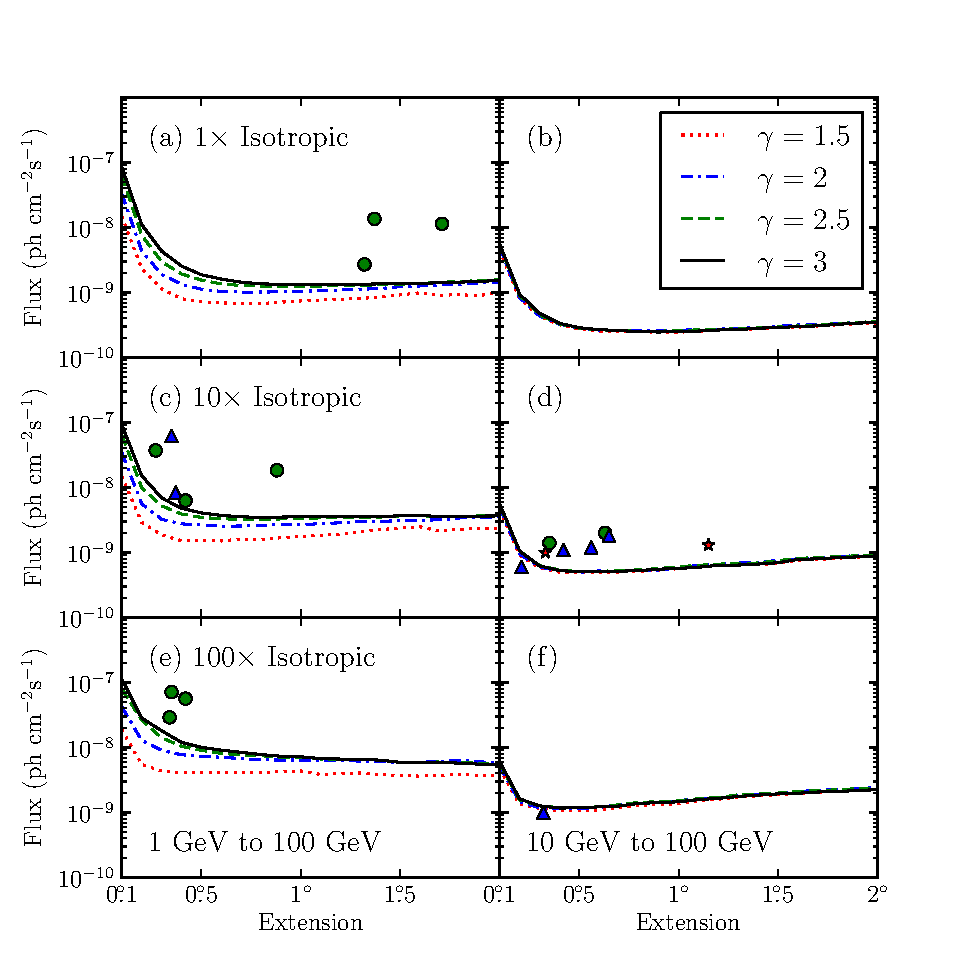
\includegraphics{mc_plots/all_sensitivity_color.pdf}
    \else
    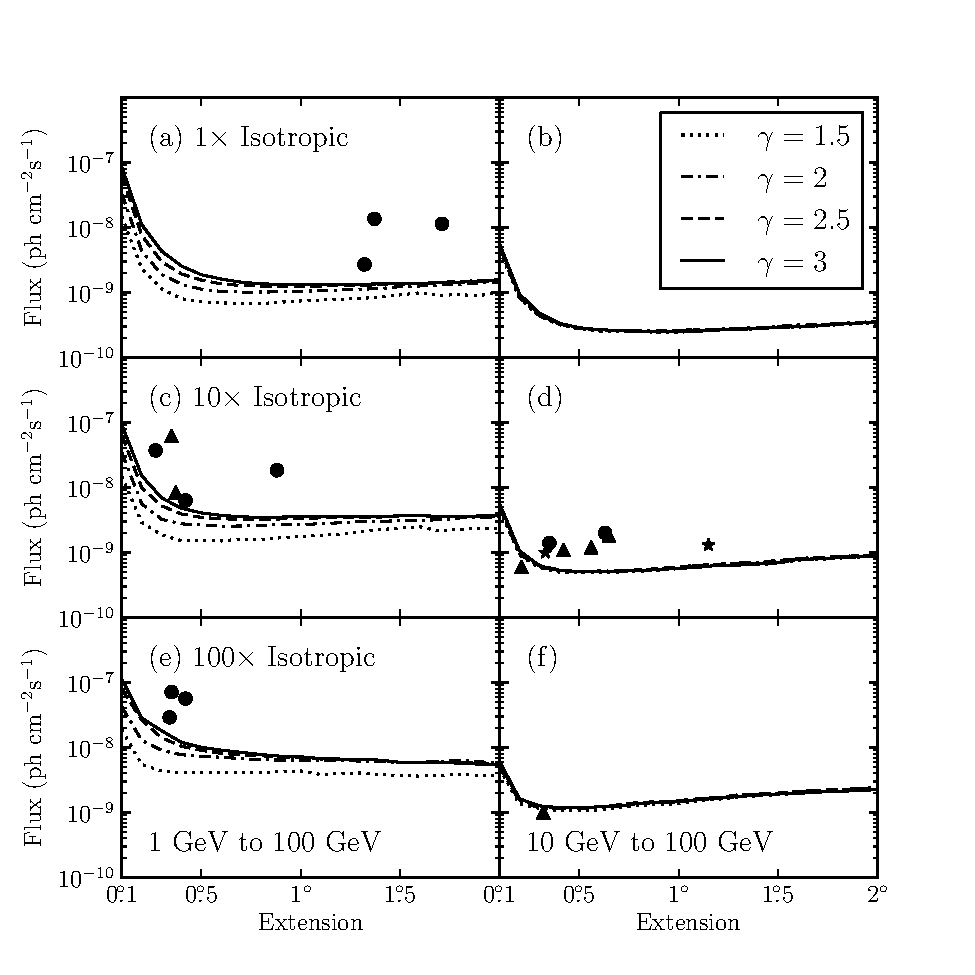
\includegraphics{mc_plots/all_sensitivity_bw.pdf}
    \fi
    \caption{The LAT detection threshold for four spectral indices
    and three backgrounds ($1\times$, $10\times$, and $100\times$ the
    Sreekumar-like isotropic background) for a two-year exposure. The
    left-hand plots are the detection threshold when using 
    photons with energies between
    1 \gev and 100 \gev
    and the right-hand plots are the detection threshold when using
    photons with energies between
    10 \gev and 100 \gev.  The flux is integrated only in the
    selected energy range.  Overlaid on this plot are the LAT-detected
    extended sources placed by the magnitude of the nearby Galactic
    diffuse emission and the energy range they were analyzed with.
    The star-shaped markers (colored red in the electronic version)
    are sources with a spectral index closer to 1.5, the triangular
    markers (colored blue) an index closer to 2, and the circular markers
    (colored green) an index closer to 2.5.  The triangular marker in plot
    (d) below the sensitivity line is MSH\,15$-$52.
    }\figlabel{all_sensitivity} 
  \end{figure}


\figref{all_sensitivity} shows the flux threshold as a function of
source extension for different background levels ($1\times$, $10\times$,
and $100\times$ the nominal background), different spectral indices,
and two different energy ranges (1 \gev to 100 \gev and 10 \gev to
100 \gev).  The detection threshold is higher for sources in regions of
higher background.  When studying sources only at energies above 1 \gev,
the LAT detection threshold (defined as the 1 \gev to 100 \gev flux at
which $\langle\tsext\rangle=16$) depends less strongly on the 
spectral index of the source. 
The index dependence of the detection threshold is
even weaker when considering only photons with energies above 10 \gev
because the PSF changes little from 10 \gev to 100 \gev.
Overlaid on \figref{all_sensitivity} are the LAT-detected extended
sources that will be discussed in \secref{validate_known} and
\secref{new_ext_srcs_section}.  The extension thresholds are tabulated in
\tabref{all_sensitivity_table}.


\begin{figure}
    \ifcolorfigure
      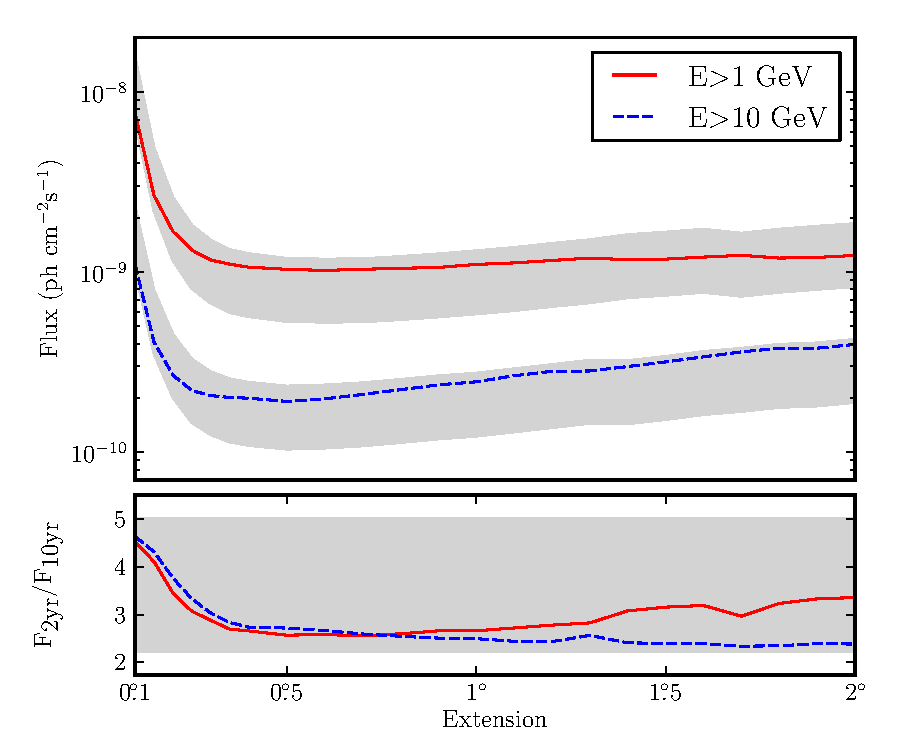
\includegraphics{mc_plots/time_sensitivity_color.pdf}
    \else
      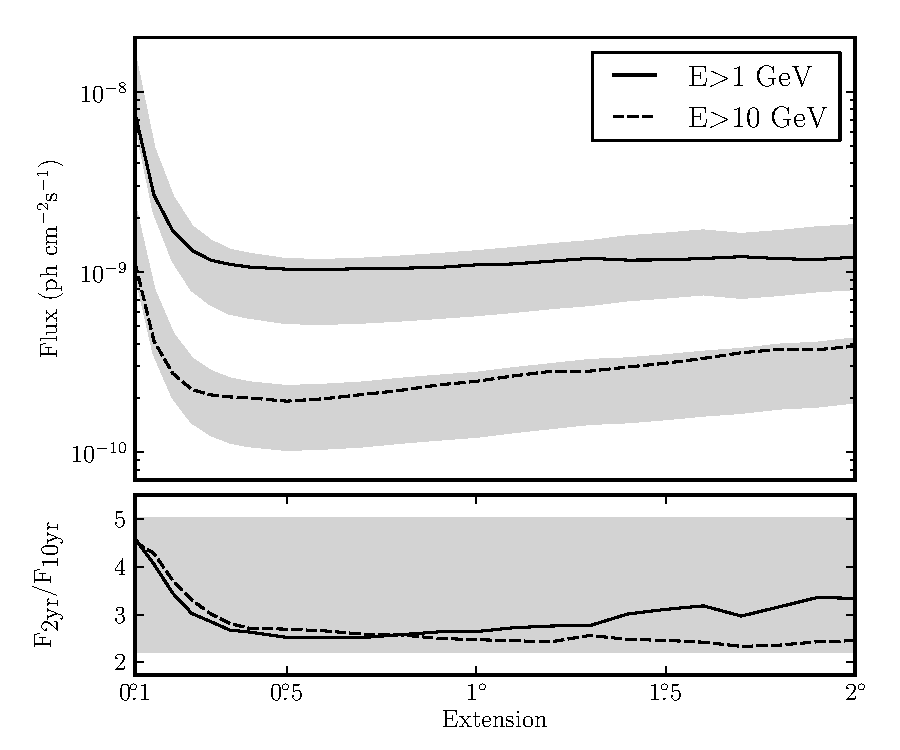
\includegraphics{mc_plots/time_sensitivity_bw.pdf}
    \fi
    \caption{
    The projected detection threshold of the LAT to extension after 10 years
    for a power-law
    source of spectral index 2 against 10 times the isotropic background
    in the energy range from 1 \gev to 100 \gev (solid line colored red in the electronic
    version) and 10 \gev to 100 \gev
    (dashed line colored blue). The shaded gray regions represent the
    detection threshold assuming the sensitivity improves from 2 to 10
    years by the square root of the exposure (top edge) and linearly with
    exposure (bottom edge).  The lower plot shows the factor increase in
    sensitivity.  For small extended sources, the detection threshold of the LAT
    to the extension of a source will improve by a factor larger than the square root of 
    the exposure.
    }\figlabel{time_sensitivity}
  \end{figure}


Finally, \figref{time_sensitivity} shows the projected
detection threshold of the LAT to extension with a 10 year
exposure against 10 times
the isotropic background measured by EGRET. This background is
representative of the background near the Galactic plane.  For small
extended sources, the threshold improves by a factor larger
than the square root of the relative exposures because the LAT is signal-limited
at high energies where the present analysis is most sensitive. For large
extended sources, the relevant background is over a larger spatial range
and so the improvement is closer to a factor corresponding
to the square root of the relative exposures that is caused by Poisson fluctuations in the background.


\section{Testing Against Source Confusion}
\seclabel{dual_localization_method}

It is impossible to discriminate using only LAT data between a
spatially extended source and multiple point-like sources separated by
angular distances comparable to or smaller than the size of the LAT PSF. 
To assess the plausibility of source confusion for sources with
$\tsext\ge16$, we developed an algorithm to test if a region contains
two point-like sources.  The algorithm works by simultaneously fitting
in \pointlike the positions and spectra of the two point-like sources.
To help with convergence, it begins by dividing the source into two
spatially coincident point-like sources and then fitting the sum and
difference of the positions of the two sources without any limitations
on the fit parameters.

After simultaneously fitting the two positions and two spectra,
we define \tsinc as twice the increase in the log of the likelihood
fitting the region with two point-like sources compared to fitting the
region with one point-like source:
\begin{equation}
  \tsinc=2\log(\likelihood_\text{2pts}/\likelihood_\text{ps}).
\end{equation} 
For the following analysis of LAT data, \tsinc was computed
by fitting the spectra of the two point-like sources in \gtlike using the best fit positions
of the sources found by \pointlike.

\tsinc cannot be quantitatively compared to \tsext using a simple
likelihood-ratio test to evaluate which model is significantly better
because the models are not nested \citep{protassov_2002a_statistics-handle}.
Even though the comparison of \tsext with \tsinc is not a calibrated
test, $\tsext>\tsinc$ indicates that the likelihood for the extended
source hypothesis is higher than for two point-like sources and we only
consider a source to be extended if $\tsext>\tsinc$.

We considered using 
the Bayesian information criterion \citep[BIC,][]{schwarz_1978a_estimating-dimension} as
an alternative Bayesian formulation for this test, but it is difficult to apply
to LAT data because it contains a term including the number of data points. 
For studying $\gamma$-ray sources in LAT data, we analyze relatively large
regions of the sky to better define the contributions from diffuse
backgrounds and nearby point sources. This is important for accurately
evaluating source locations and fluxes but the fraction of data directly
relevant to the evaluation of the parameters for the source of interest
is relatively small.

As an alternative, we considered the Akaike information criterion test \citep[\aic,][]{akaike_1974a_statistical-model}.
The \aic is defined as $\aic=2k-2\log\likelihood$, where $k$ is the number of parameters in the model. 
In this formulation, the best hypothesis is considered to be the one that minimizes the \aic.
The first term penalizes models with additional parameters. 

The two point-like sources hypothesis has three more parameters than
the single extended source hypothesis (two more spatial parameters and
two more spectral parameters compared to one extension parameter), so the
comparison $\aic_\text{ext} < \aic_\text{2pts}$  is formally equivalent to
$\tsext + 6 > \tsinc$.  Our criterion for accepting extension ($\tsext > \tsinc$) 
is thus equivalent to requesting that the AIC-based empirical
support for the two point-like sources model be ``considerably less''
than for the extended source model, following the classification by
\cite{burnham_2002a_model-selection}.

We assessed the power of the $\tsext>\tsinc$ test with a Monte Carlo
study.  We simulated one spatially extended source and fit it as both
an extended source and as two point-like sources using \pointlike.
We then simulated two point-like sources and fit them with the same two
hypotheses. By comparing the distribution of \tsinc and \tsext computed by
\pointlike for the two cases, we evaluated how effective the $\tsext>\tsinc$
test is at rejecting cases of source confusion as well as how
likely it is to incorrectly reject that an extended source is spatially
extended.  All sources were simulated using the same time range as in
\subsecref{extension_sensitivity} against a background 10 times the
isotropic background measured by EGRET, representative of the background
near the Galactic plane.

\clearpage
\begin{figure}
    \ifcolorfigure
    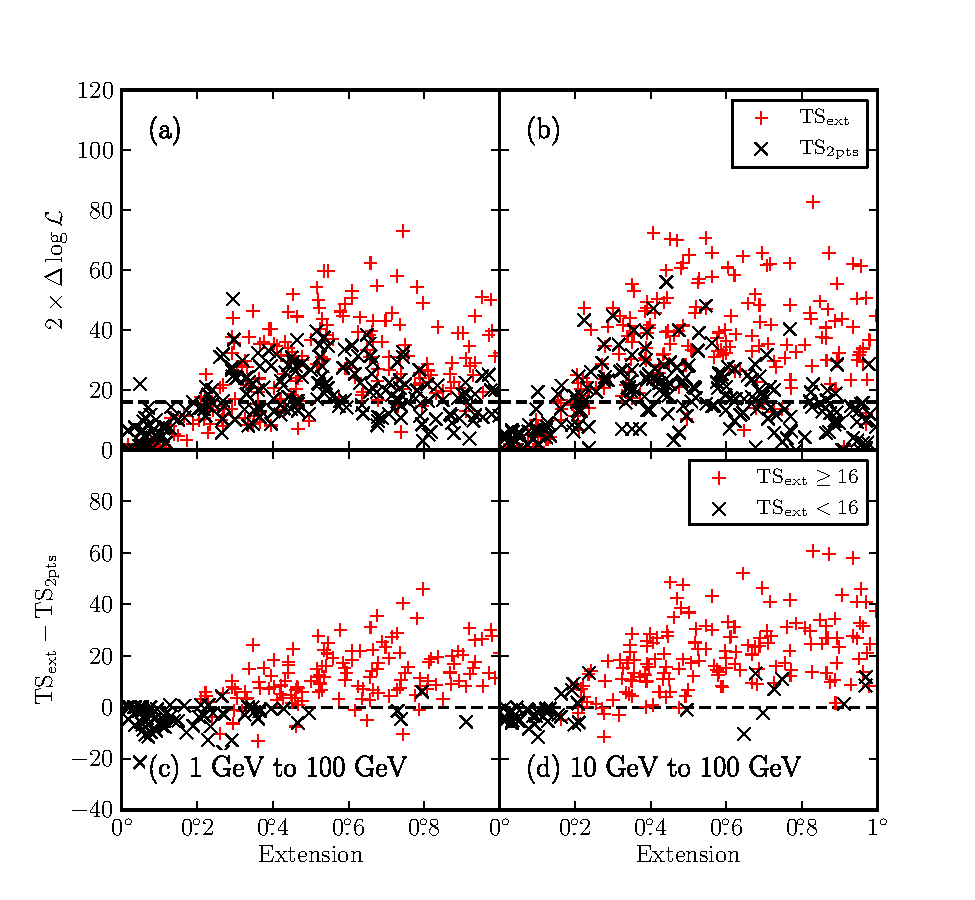
\includegraphics{mc_plots/confusion_extended_plot_color.pdf}
    \else
    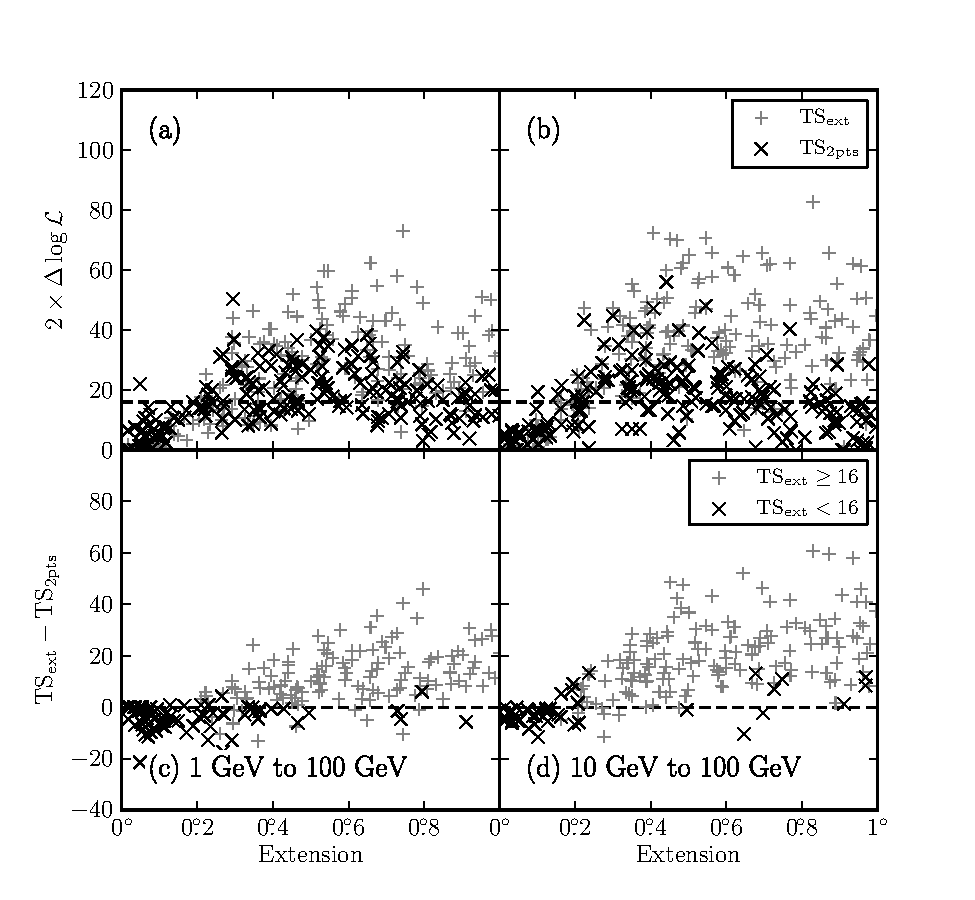
\includegraphics{mc_plots/confusion_extended_plot_bw.pdf}
    \fi
    \caption{
    (a) and (b) are the distribution of \tsext and of \tsinc when
    fitting simulated spatially extended sources of varying sizes as
    both an extended source and as two point-like sources.  (c) and
    (d) are the distribution of $\tsext-\tsinc$ for the same simulated sources.
    (a) and (c) represent sources fit in the 1 \gev to 100 \gev energy
    range and (b) and (d) represent sources fit in the 10 \gev to
    100 \gev energy range.  In (c) and (d), the plus-shaped markers
    (colored red in the electronic version) are fits where $\tsext\ge16$.
    }\figlabel{confusion_extended_plot}
  \end{figure}




We did this study first in the energy range from 1 \gev to 100 \gev by
simulating extended sources of flux $4\times10^{-9}$ \fluxunits integrated
from 1 \gev to 100 \gev and a power-law spectral model with
spectral index 2.  This spectrum was picked to be representative of the
new extended sources that were discovered in the following analysis
when looking in the 1 \gev to 100 \gev energy range
(see \secref{new_ext_srcs_section}).
We simulated these sources using uniform disk spatial models
with extensions varying
up to $1\degree$.  
\figref{confusion_extended_plot}a shows the distribution
of \tsext and \tsinc and 
\figref{confusion_extended_plot}c shows 
the distribution of $\tsext-\tsinc$ as a
function of the simulated extension of the source
for 200 statistically independent simulations.


\clearpage
\begin{figure}
    \ifcolorfigure
    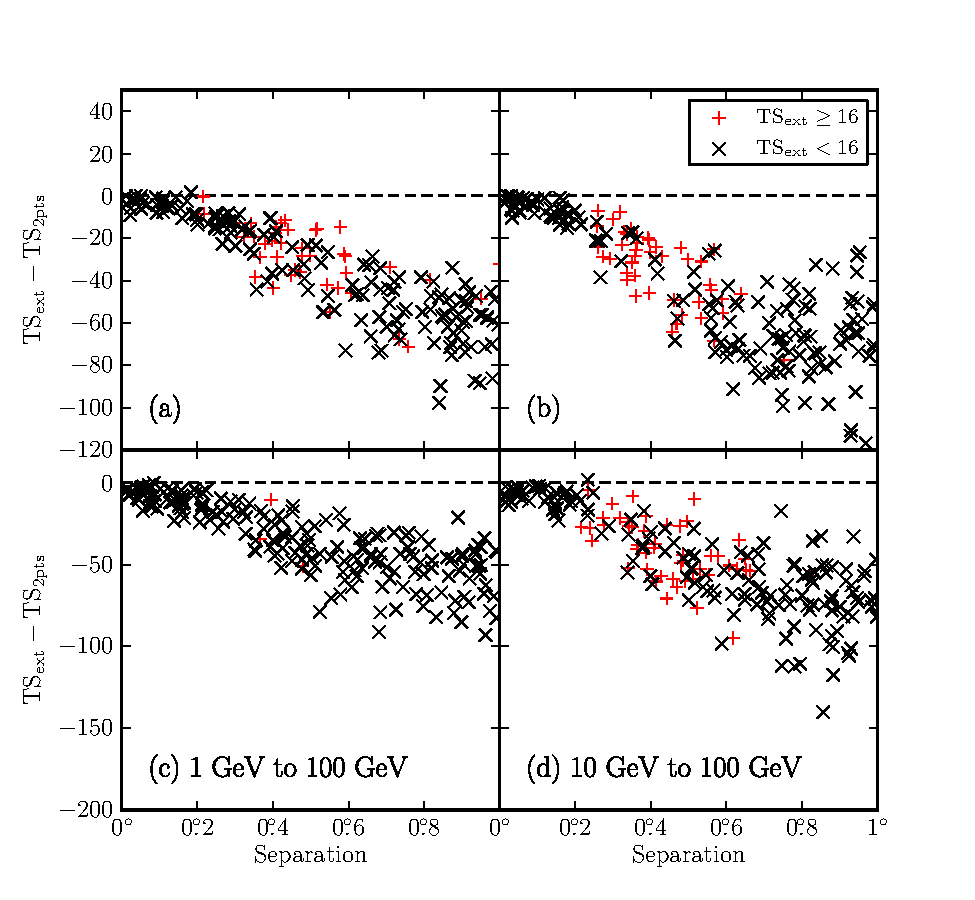
\includegraphics{mc_plots/confusion_2pts_plot_color.pdf}
    \else
    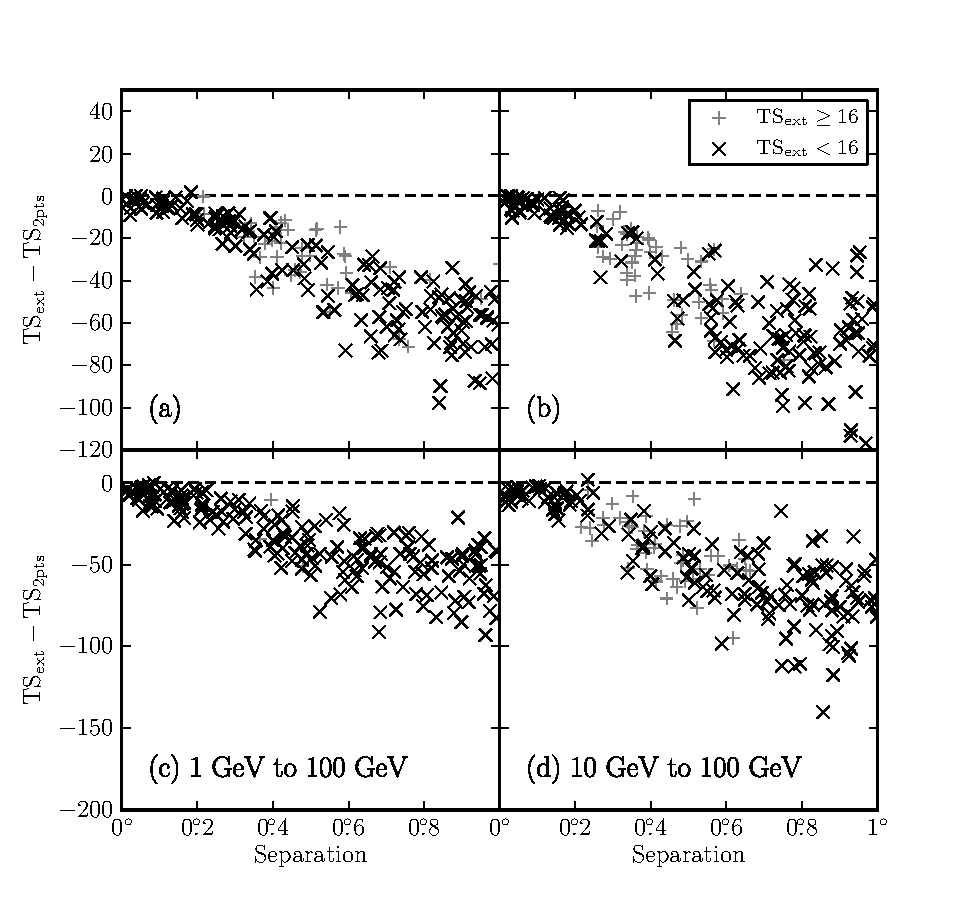
\includegraphics{mc_plots/confusion_2pts_plot_bw.pdf}
    \fi
    \caption{
    The distribution of $\tsext-\tsinc$ when fitting two simulated
    point-like sources of varying separations as
    both an extended source and as two point-like sources.  (a),
    and (b) represent simulations of two point-like sources with the
    same spectral index and (c) and (d) represent simulations of two
    point-like sources with different spectral indices.  (a) and (c)
    fit the simulated sources in the 1 \gev to 100 \gev energy range
    and (b) and (d) fit in the 10 \gev to 100 \gev energy range.
    The plus-shaped markers (colored red in the electronic version)
    are fits where $\tsext\ge16$.
    }\figlabel{confusion_2pts_plot}
  \end{figure}

\figref{confusion_2pts_plot}a shows the same plot but when fitting
two simulated point-like sources each with half of the flux of
the spatially extended source and with the same spectral index as the
extended source.  Finally, \figref{confusion_2pts_plot}c shows the same
plot with each point-like source having the same flux but different
spectral indices.  One point-like source had a spectral index of 1.5
and the other an index of 2.5.
These indices are representative of the range of indices of LAT-detected
sources.

The same four plots are shown in \figref{confusion_extended_plot}b, \figref{confusion_extended_plot}d, 
\figref{confusion_2pts_plot}b, and \figref{confusion_2pts_plot}d but this
time when analyzing a source of flux $10^{-9}$ \fluxunits (integrated from
10 \gev to 100 \gev) only in the 10 \gev to 100 \gev energy range.
This flux is typical of the new extended sources discovered
using only photons with energies between 10 \gev and 100 \gev (see
\secref{new_ext_srcs_section}).

Several interesting conclusions can be made from this study.  As one would
expect, $\tsext-\tsinc$ is mostly positive when fitting the simulated
extended sources.  In the 1 \gev to 100 \gev analysis, only 11 of the
200 simulated extended sources had $\tsext>16$ but were incorrectly
rejected due to \tsinc being greater than \tsext.  In the 10 \gev to 100 \gev
analysis, only 7 of the 200 sources were incorrectly rejected. From this,
we conclude that this test is unlikely to incorrectly reject truly
spatially extended sources.

On the other hand, 
it is often
the case that $\tsext>16$ when testing the 
two simulated point-like sources
for extension.  This is especially the case
when the two sources had the same spectral index. Forty out of 200 sources
in the 1 \gev to 100 \gev energy range and 43 out of 200 sources in the
10 \gev to 100 \gev energy range had $\tsext>16$.  But in these cases,
we always found the single extended source fit to be worse than
the two point-like source fit.  From this, we conclude that the $\tsext>\tsinc$
test is powerful at discarding cases in which the true emission comes
from two point-like sources.


The other interesting feature in \figref{confusion_extended_plot}a
and \figref{confusion_extended_plot}b is that for simulated extended
sources with typical sizes ($\sigma\sim0\fdg5$), one can often obtain
almost as large an increase in likelihood fitting the source as two
point-like sources ($\tsinc\sim\tsext$).  This is because although the
two point-like sources represent an incorrect spatial model, the second
source has four additional degrees of freedom (two spatial and two
spectral parameters) and can therefore easily model much of the extended
source and statistical fluctuations in the data.  This effect is most
pronounced when using photons with energies between 1 \gev and 100 \gev
where the PSF is broader.

From this Monte Carlo study, we can see the limits of an analysis with
LAT data of spatially extended sources.  \subsecref{monte_carlo_validation}
showed that we have a statistical test that finds when a LAT source is
not well described by the PSF.  But this test does not uniquely prove
that the emission originates from spatially extended emission instead
of from multiple unresolved sources.  Demanding that $\tsext>\tsinc$
is a powerful second test to avoid cases of simple confusion of two
point-like sources. But it could always be the case that an extended
source is actually the superposition of multiple point-like or
extended sources that could be resolved with deeper observations of the
region.  There is nothing about this conclusion unique to analyzing LAT data,
but the broad PSF of the LAT and the density of sources expected to be
\gev emitters in the Galactic plane makes this issue more significant
for analyses of LAT data.  When possible, multiwavelength information should be
used to help select the best model of the sky.


\section{Test of 2LAC Sources}
\seclabel{test_2lac_sources}


For all following analyses of LAT data, we used the same two-year dataset
that was used in the 2FGL catalog spanning from 2008 August 4 to 2010 August 1. We
applied the same acceptance cuts and we used the same P7\_V6 Source class
event selection and IRFs \citep{ackermann_2012a_fermi-large}.  
When analyzing sources in \pointlike, we used a circular $10\degree$ region of
interest (ROI) centered on our source and eight energy bins per
logarithmic decade in energy.
When refitting the region in \gtlike using the best fit spatial and
spectral models from \pointlike, we used the `binned likelihood' mode of
\gtlike on a $14\degree\times14\degree$ ROI with a pixel size of 0\fdg03.

Unless explicitly
mentioned, we used the same background model as 2FGL to represent the
Galactic diffuse, isotropic, and Earth limb emission.  To compensate for
possible residuals in the diffuse emission model, the Galactic emission
was scaled by a power-law and the normalization
of the isotropic component
was left free.  
Unless explicitly mentioned,
we used all 2FGL sources within $15\degree$ of our source as our list
of background sources and we refit the spectral parameters of all sources
within $2\degree$ of the source.



To validate our method, we tested LAT sources associated with AGN for
extension.  \gev emission from AGN is believed to originate from collimated jets.  Therefore AGN are
not expected to be spatially resolvable by the LAT and provide a good
calibration source to demonstrate that our extension detection method
does not misidentify point-like sources as being extended.  We note that
megaparsec-scale $\gamma$-ray halos around AGNs have been hypothesized
to be resolvable by the LAT \citep{aharonian_1994a_energy-gamma}. However, no such
halo has been discovered in the LAT data so far \citep{neronov_2011a_evidence-gamma-ray}.

Following 2FGL, the LAT Collaboration published the Second LAT AGN
Catalog (2LAC), a list of high latitude ($|b|>10\degree$) sources
that had a high probability association with AGN \citep{ackermann_2011a_second-catalog}.
2LAC associated 1016 2FGL sources with AGN.  To avoid systematic problems
with AGN classification, we selected only the 885 AGN which made it into
the clean AGN sub-sample defined in the 2LAC paper.  An AGN association is considered clean only
if it has a high probability of association $P\ge 80\%$, if it is the
only AGN associated with the 2FGL source, and if 
no analysis flags have been set for the source
in the 2FGL catalog. These last two conditions are important for our
analysis. Source confusion may look like a spatially extended source
and flagged 2FGL sources may correlate with unmodeled structure in
the diffuse emission.

\clearpage
\begin{figure}
    \ifcolorfigure
      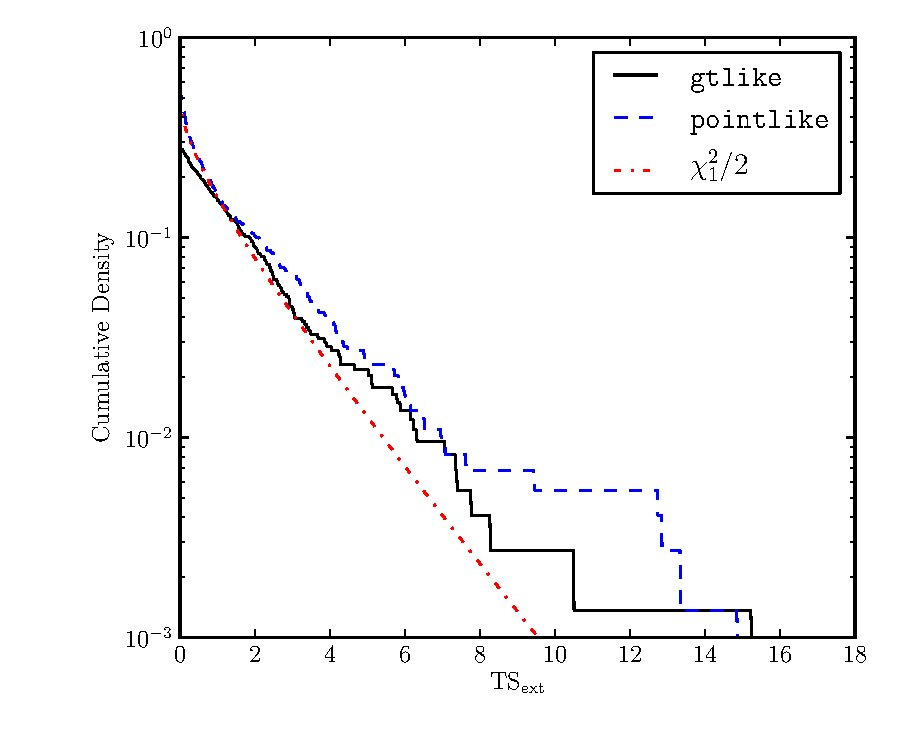
\includegraphics{source_plots/agn_color.pdf}
    \else
      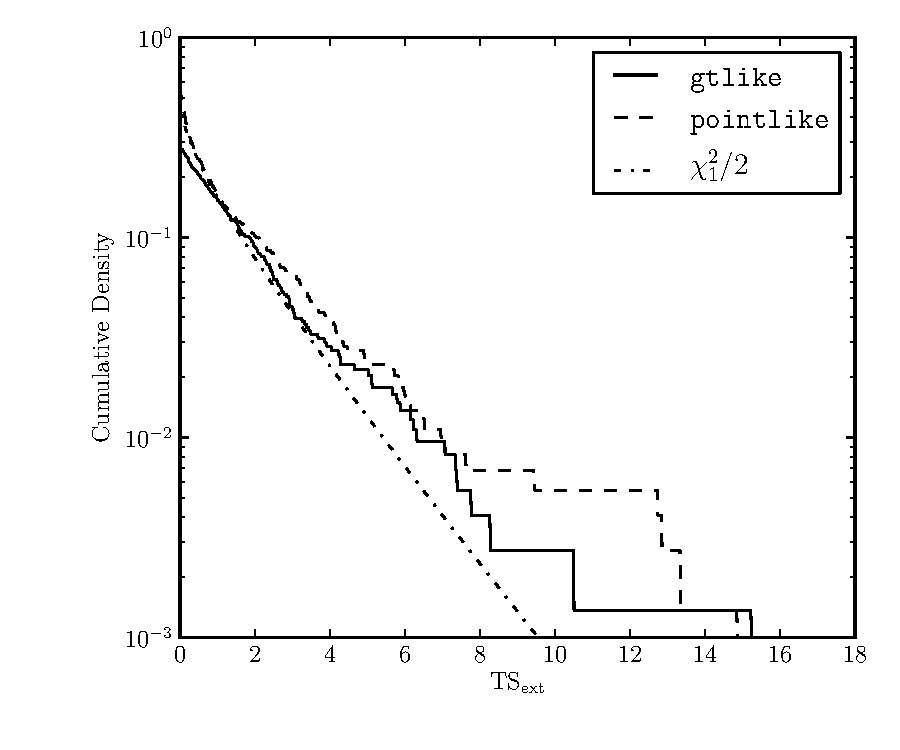
\includegraphics{source_plots/agn_bw.pdf}
    \fi
    \caption{The cumulative density of \tsext for the 733 clean
    AGN in 2LAC that were significant above 1 \gev calculated with \pointlike (dashed line
    colored blue in the electronic version)
    and with \gtlike (solid line colored black).  AGN are too far
    and too small to be resolved by the LAT. Therefore, the cumulative
    density of $\tsext$ is expected to follow a $\chi^2_1/2$ distribution
    (\eqnref{ts_ext_distribution}, the dash-dotted line colored
    red).
    }\figlabel{agn_ts_ext}
  \end{figure}



Of the 885 clean AGN, we selected the 733 of these 2FGL sources which
were significantly detected above 1 \gev and fit each of them for
extension.  The cumulative density of \tsext for these AGN is compared
to the $\chi^2_1/2$ distribution of \eqnref{ts_ext_distribution}
in \figref{agn_ts_ext}.  The \tsext distribution
for the AGN shows reasonable agreement with the theoretical
distribution and no AGN was found to be significantly extended
($\tsext>16$).  The observed discrepancy from the theoretical
distribution is likely due to small systematics
in our model of the LAT PSF and the Galactic diffuse emission (see
\secref{systematic_errors_on_extension}).  
The discrepancy could
also in a few cases be due to confusion with a nearby undetected source.
We note that the Monte Carlo study
of \subsecref{monte_carlo_validation} effectively used perfect
IRFs and a perfect model of the sky.
The overall agreement with the expected distribution demonstrates that
we can use \tsext as a measure of the statistical significance of the
detection of the extension of a source.

We note that the LAT PSF used in this study was determined
empirically by fitting the distributions of gamma rays around bright AGN (see
\secref{systematic_errors_on_extension}). Finding that the AGN we
test are not extended is not surprising.  This validation analysis is
not suitable to reject any hypotheses about the existence of megaparsec-scale
halos around AGN.

